\documentclass[10pt]{beamer}

\usetheme{Madrid}
\usecolortheme{default}
\setbeamertemplate{navigation symbols}{}
\setbeamersize{text margin left=0.6cm,text margin right=0.6cm}

\usepackage{amsmath,amssymb}
\usepackage{tikz}
\usepackage{tikz-qtree}
\usetikzlibrary{arrows.meta,positioning,calc}
\usepackage{booktabs}
\usepackage{array}

\newcolumntype{L}[1]{>{\raggedright\arraybackslash}p{#1}}
\pdfstringdefDisableCommands{\def\translate#1{#1}}
\newcommand{\paperlink}[2]{%
  \href{#1}{\textcolor{blue!65!black}{#2}}%
}
\setbeamercovered{transparent=18}

\title{Context-Free Grammars}
\subtitle{Derivations, Normal Forms, Properties, and Pumping}
\author{Computer Science Theory}
\date{Slide Set 5}

\begin{document}

\begin{frame}
  \titlepage
\end{frame}

\begin{frame}{Learning Outcomes}
  \small
  By the end of this slide set, you should be able to:
  \begin{itemize}
    \item define a context-free grammar (CFG) and the language it generates;
    \item distinguish sentential forms, sentences, and leftmost/rightmost derivations;
    \item prove that a proposed grammar generates exactly a specified language;
    \item define complete and partial derivation trees and compute their frontiers;
    \item demonstrate ambiguity using parse trees or leftmost derivations;
    \item recognize $s$-grammars and explain their predictive behavior;
    \item eliminate null, unit, and useless productions from a CFG;
    \item convert grammars to CNF and GNF and distinguish the two forms;
    \item apply CYK, analyze its complexity, and distinguish major extensions
      from alternative parsing algorithms;
    \item state the principal closure and decision properties of CFLs;
    \item use the CFL pumping lemma to prove languages non-context-free;
    \item rewrite grammars for precedence and express syntax using BNF/EBNF.
  \end{itemize}
\end{frame}

\begin{frame}{Road Map}
  \tableofcontents
\end{frame}

% ==========================================
% Part 1: Motivation
% ==========================================
\section{Motivation: Recursive Structure}

\begin{frame}{Why Context-Free Grammars?}
  Finite automata recognize patterns using only finite memory. They cannot enforce an unbounded
  exact match such as
  \[
    \{0^n1^n\mid n\ge0\}.
  \]
  A CFG describes a language \emph{generatively}: it recursively builds valid strings from a start
  variable.
  \pause
  \begin{block}{What recursion gives us}
    A finite set of productions can describe arbitrarily deep nesting, matched delimiters,
    recursive program syntax, and self-similar structure.
  \end{block}
  \pause
  \begin{alertblock}{Power and limitation}
    Every regular language is context-free, but some languages---for example
    $\{a^n b^n c^n\mid n\ge0\}$---are not context-free.
  \end{alertblock}
\end{frame}

\begin{frame}{An Inductive Definition: Balanced Parentheses}
  A balanced-parenthesis string can be defined recursively:
  \begin{enumerate}
    \item the empty string is balanced;
    \item if $x$ and $y$ are balanced, then $(x)y$ is balanced; and
    \item nothing else is balanced.
  \end{enumerate}
  \pause
  This becomes the grammar
  \[
    S\to (S)S\mid\varepsilon.
  \]
  \pause
  \begin{exampleblock}{Examples}
    \[
      \varepsilon,\quad (),\quad (()),\quad ()(),\quad (()())
    \]
  \end{exampleblock}
  The first $S$ creates nesting inside a pair; the second permits another balanced string to follow.
\end{frame}

% ==========================================
% Part 2: Formal Definition
% ==========================================
\section{Definition and Derivations}

\begin{frame}{Formal Definition of a CFG}
  We use the Linz-style notation $G=(V,T,S,P)$. Sipser commonly writes
  $(V,\Sigma,R,S)$; the components are the same up to names and order.
  \pause
  \begin{block}{Definition}
    A context-free grammar is a 4-tuple $G=(V,T,S,P)$, where:
    \begin{enumerate}
      \item $V$ is a finite set of variables (nonterminals);
      \item $T$ is a finite set of terminals, with $V\cap T=\varnothing$;
      \item $S\in V$ is the start variable; and
      \item $P$ is a finite set of productions $A\to\alpha$, where
        $A\in V$ and $\alpha\in(V\cup T)^*$.
    \end{enumerate}
  \end{block}
  Alternatives such as $A\to x$, $A\to y$, and $A\to z$ are abbreviated
  $A\to x\mid y\mid z$.
\end{frame}

\begin{frame}{What Does ``Context-Free'' Mean?}
  A production has exactly one variable on its left-hand side:
  \[
    A\to\alpha.
  \]
  Therefore $A$ may be replaced by $\alpha$ regardless of the symbols surrounding it.
  \pause
  \begin{center}
  \begin{tabular}{L{4.5cm}L{5.3cm}}
    \toprule
    Valid CFG productions & Not CFG productions \\
    \midrule
    $S\to 0S1$ & $AB\to BA$ (two variables on the left) \\
    $A\to aB\mid\varepsilon$ & $aA\to Aa$ (a terminal occurs on the left) \\
    $B\to C$ & $\varepsilon\to S$ (no variable on the left) \\
    \bottomrule
  \end{tabular}
  \end{center}
  \begin{alertblock}{Terminology}
    ``Context-free'' describes the form of the productions. It does not mean that the generated
    strings lack structure or context.
  \end{alertblock}
\end{frame}

\begin{frame}{Derivations and Sentential Forms}
  If $A\to\alpha$ is a production, then for any $u,v\in(V\cup T)^*$,
  \[
    uAv\Rightarrow u\alpha v.
  \]
  \begin{itemize}
    \item $\Rightarrow$: one derivation step;
    \item $\Rightarrow^*$: zero or more steps;
    \item $\Rightarrow^+$: one or more steps;
    \item \textbf{sentential form}: any $\gamma$ such that $S\Rightarrow^*\gamma$;
    \item \textbf{sentence}: a terminal-only sentential form $w\in T^*$.
  \end{itemize}
  \pause
  The generated language is
  \[
    L(G)=\{w\in T^*\mid S\Rightarrow^*w\}.
  \]
  Because $\Rightarrow^*$ allows zero steps, $S$ itself is a sentential form but normally not a sentence.
\end{frame}

\begin{frame}{Leftmost and Rightmost Derivations}
  Consider
  \[
    S\to AB,\qquad A\to aA\mid a,\qquad B\to bB\mid b.
  \]
  A leftmost derivation of $aabb$ is
  \[
    S\Rightarrow AB\Rightarrow aAB\Rightarrow aaB
      \Rightarrow aabB\Rightarrow aabb.
  \]
  \pause
  A rightmost derivation of the same string is
  \[
    S\Rightarrow AB\Rightarrow AbB\Rightarrow Abb
      \Rightarrow aAbb\Rightarrow aabb.
  \]
  \begin{block}{Key point}
    The replacement order differs, but both derivations describe the same hierarchical parse tree.
    Derivation order alone is not semantic structure.
  \end{block}
\end{frame}

\begin{frame}{Proving What a Grammar Generates}
  For
  \[
    G:\quad S\to0S1\mid\varepsilon,
  \]
  prove $L(G)=\{0^n1^n\mid n\ge0\}$ using two inclusions.
  \begin{block}{Soundness: $L(G)\subseteq\{0^n1^n\}$}
    Every use of $S\to0S1$ adds one $0$ to the left and one $1$ to the right.
    After $k$ such steps the form is $0^kS1^k$; replacing $S$ by $\varepsilon$
    yields $0^k1^k$.
  \end{block}
  \pause
  \begin{block}{Completeness: $\{0^n1^n\}\subseteq L(G)$}
    For any $n\ge0$, apply $S\to0S1$ exactly $n$ times and then
    $S\to\varepsilon$:
    $S\Rightarrow^*0^nS1^n\Rightarrow0^n1^n$.
  \end{block}
  Testing examples suggests a grammar; the two-inclusion argument proves it.
\end{frame}

\begin{frame}{Reusable Grammar-Design Patterns I}
  \begin{columns}[T]
    \column{0.32\textwidth}
    \begin{block}{Matched Blocks}
      \[
        S\to0S1\mid\varepsilon
      \]
      Generates $0^n1^n$ by adding matched symbols at opposite ends.
    \end{block}

    \column{0.32\textwidth}
    \begin{block}{Palindromes}
      \[
        S\to0S0\mid1S1\mid0\mid1\mid\varepsilon
      \]
      Add the same symbol to both ends; base cases determine parity.
    \end{block}

    \column{0.32\textwidth}
    \begin{block}{Balanced Strings}
      \[
        S\to(S)S\mid\varepsilon
      \]
      One variable position handles nesting and the other concatenation.
    \end{block}
  \end{columns}
\end{frame}

\begin{frame}{Informal Preview: One String, Two Structures}
  \small
  Before giving the formal definition, it is useful to recognize the problem
  informally. A grammar can sometimes generate the same terminal string with
  two genuinely different hierarchical meanings.
  \pause
  \begin{exampleblock}{Arithmetic preview}
    The string
    \[
      \mathrm{id}+\mathrm{id}\times\mathrm{id}
    \]
    might mean either
    \[
      (\mathrm{id}+\mathrm{id})\times\mathrm{id}
      \qquad\text{or}\qquad
      \mathrm{id}+(\mathrm{id}\times\mathrm{id}).
    \]
  \end{exampleblock}
  \pause
  This is called \textbf{structural ambiguity}: the sequence of terminals is
  fixed, but its parse-tree structure is not. Later we will define ambiguity
  formally and rewrite the grammar to encode precedence and associativity.
  \begin{alertblock}{Why this preview matters}
    Earlier grammar constructions may offer several production choices. That
    is not automatically a problem; ambiguity occurs only when choices give
    two different structures for the \emph{same} string.
  \end{alertblock}
\end{frame}

\begin{frame}{Reusable Grammar-Design Patterns II}
  Suppose grammars with renamed, disjoint variables generate $L_1$ and $L_2$ from start variables
  $S_1$ and $S_2$.
  \begin{center}
  \begin{tabular}{L{3.0cm}L{3.6cm}L{3.3cm}}
    \toprule
    Goal & New start production & Meaning \\
    \midrule
    $L_1\cup L_2$ & $S\to S_1\mid S_2$ & choose either grammar \\
    $L_1L_2$ & $S\to S_1S_2$ & generate one string from each \\
    $L_1^*$ & $S\to S_1S\mid\varepsilon$ & repeat zero or more times \\
    \bottomrule
  \end{tabular}
  \end{center}
  \pause
  \begin{alertblock}{Language generation versus ambiguity}
    These constructions generate the intended languages, but they may produce ambiguous grammars
    when a string can be decomposed in more than one way.
  \end{alertblock}
\end{frame}

\begin{frame}{A Grammar-Design Workflow}
  \begin{enumerate}
    \item Identify the recursive or nested structure of valid strings.
    \item Choose one variable for each meaningful syntactic category or phase.
    \item Write recursive productions that preserve the required invariant.
    \item Add base cases so the recursion can terminate.
    \item Test the smallest valid strings and several invalid strings.
    \item Prove both soundness and completeness.
    \item Check whether the grammar accidentally introduces ambiguity.
  \end{enumerate}
  \pause
  \begin{block}{Debugging question}
    If an invalid string is generated, which production allowed the invariant to break? If a valid
    string is missing, which necessary base case or recursive choice is absent?
  \end{block}
\end{frame}

% ==========================================
% Part 3: Parse Trees
% ==========================================
\section{Parse Trees}

\begin{frame}{Formal Definition of a Derivation Tree}
  \small
  A \textbf{derivation tree} (parse tree) for $G=(V,T,S,P)$ is a finite,
  rooted, ordered tree satisfying:
  \begin{enumerate}
    \item the root is labeled $S$;
    \item every internal node is labeled by a variable;
    \item if a node labeled $A$ has children
      $X_1,\ldots,X_k$ from left to right, then
      $A\to X_1\cdots X_k\in P$; and
    \item every leaf is labeled by a terminal or by $\varepsilon$.
  \end{enumerate}
  \begin{columns}[T]
    \column{0.55\textwidth}
    The \textbf{yield} is obtained by reading the leaves from left to right
    and omitting $\varepsilon$.
    \begin{block}{Derivation-tree theorem}
      $S\Rightarrow^*w$ for $w\in T^*$ iff a derivation tree rooted at $S$
      has yield $w$.
    \end{block}
    \column{0.40\textwidth}
    \centering
    \begin{tikzpicture}[sibling distance=18pt,level distance=21pt,
      every node/.style={font=\small}]
      \Tree [.S a [.S $\varepsilon$ ] b ]
    \end{tikzpicture}

    Yield: $ab$
  \end{columns}
\end{frame}

\begin{frame}{Partial Derivation Trees and Sentential Forms}
  \small
  A \textbf{partial derivation tree} obeys the same root and production
  conditions, but some leaves may still be variables. Its
  \textbf{frontier} is the left-to-right sequence of terminal and variable
  leaves, with $\varepsilon$ omitted.
  \begin{block}{Formal correspondence}
    For every $\alpha\in(V\cup T)^*$,
    \[
      S\Rightarrow^*\alpha
      \quad\Longleftrightarrow\quad
      \text{some partial derivation tree has frontier }\alpha.
    \]
  \end{block}
  \begin{columns}[T]
    \column{0.44\textwidth}
    \centering\textbf{Partial tree}

    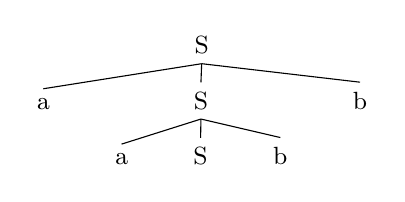
\begin{tikzpicture}[sibling distance=17pt,level distance=20pt,
      every node/.style={font=\small}]
      \Tree [.S a [.S a [.S ] b ] b ]
    \end{tikzpicture}

    Frontier: $aaSbb$
    \column{0.10\textwidth}
    \centering
    \vspace{1.1cm}
    $\Longrightarrow$
    \column{0.44\textwidth}
    \centering\textbf{Completed tree}

    \begin{tikzpicture}[sibling distance=17pt,level distance=20pt,
      every node/.style={font=\small}]
      \Tree [.S a [.S a [.S $\varepsilon$ ] b ] b ]
    \end{tikzpicture}

    Yield: $aabb$
  \end{columns}
\end{frame}

\begin{frame}{Worked Parse Tree for $aabb$}
  Grammar: $S\to aSb\mid\varepsilon$.
  \begin{columns}[T]
    \column{0.45\textwidth}
    \textbf{Derivation}
    \[
      S\Rightarrow aSb
       \Rightarrow aaSbb
       \Rightarrow aabb.
    \]
    Each internal $S$ node records one selected production.

    \column{0.52\textwidth}
    \centering
    \begin{tikzpicture}[sibling distance=22pt,level distance=25pt]
      \Tree [.S a [.S a [.S $\varepsilon$ ] b ] b ]
    \end{tikzpicture}
  \end{columns}
  \vspace{0.25cm}
  Reading the leaves gives $aa\varepsilon bb$, whose yield is $aabb$.
\end{frame}

\begin{frame}{What Is an Abstract Syntax Tree?}
  \small
  An \textbf{abstract syntax tree (AST)} is a compact tree representation of
  the essential constructs in a parsed input. Unlike a derivation tree, an AST
  is a compiler-design data structure rather than part of the formal
  definition of a CFG.
  \pause
  \begin{columns}[T]
    \column{0.47\textwidth}
    \begin{block}{A parse tree retains}
      \begin{itemize}
        \item grammar variables such as $E,T,F$;
        \item punctuation and delimiters;
        \item every production application; and
        \item helper symbols introduced for parsing.
      \end{itemize}
    \end{block}
    \column{0.47\textwidth}
    \begin{block}{An AST retains}
      \begin{itemize}
        \item operators and operands;
        \item declarations and statements;
        \item nesting and evaluation structure; and
        \item source locations needed for diagnostics.
      \end{itemize}
    \end{block}
  \end{columns}
  \pause
  Different concrete grammars can be translated into the same AST design,
  allowing later compiler phases to remain independent of parsing details.
\end{frame}

\begin{frame}{Derivation Order Versus Tree Structure}
  Suppose a sentential form contains several variables. Expanding the left one first or the right one
  first may produce different step sequences but the same tree.
  \begin{block}{Correspondence theorem}
    Every parse tree determines exactly one leftmost derivation and exactly one rightmost derivation.
  \end{block}
  Consequently:
  \begin{itemize}
    \item two distinct arbitrary derivations do \emph{not} necessarily prove ambiguity;
    \item two distinct leftmost derivations of the same string do prove ambiguity; and
    \item two distinct parse trees of the same string are the clearest structural proof.
  \end{itemize}
  This distinction prevents one of the most common mistakes in CFG exercises.
\end{frame}

\begin{frame}{Worked AST Example: $x+2\times y$}
  \small
  Suppose the expression grammar enforces multiplication precedence over
  addition. The detailed parse tree and its AST record the same essential
  grouping at different abstraction levels.
  \pause
  \begin{columns}[T]
    \column{0.56\textwidth}
    \centering\textbf{Derivation/parse tree}

    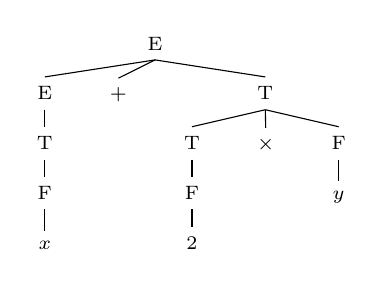
\begin{tikzpicture}[sibling distance=14pt,level distance=18pt,
      every node/.style={font=\scriptsize}]
      \Tree [.E
        [.E [.T [.F $x$ ] ] ]
        $+$
        [.T
          [.T [.F $2$ ] ]
          $\times$
          [.F $y$ ]
        ]
      ]
    \end{tikzpicture}
    \column{0.40\textwidth}
    \centering\textbf{Abstract syntax tree}

    \begin{tikzpicture}[sibling distance=28pt,level distance=25pt,
      every node/.style={font=\small}]
      \Tree [.$+$
        $x$
        [.$\times$ $2$ $y$ ]
      ]
    \end{tikzpicture}
  \end{columns}
  \pause
  \begin{block}{AST representation}
    The AST is $+(x,\times(2,y))$. Variables $E,T,F$ disappear, while the
    operator hierarchy remains explicit for type checking, optimization, and
    code generation.
  \end{block}
\end{frame}

% ==========================================
% Part 4: Ambiguity
% ==========================================
\section{Ambiguity}

\begin{frame}{What Is an Ambiguous Grammar?}
  \begin{block}{Definition}
    A CFG is ambiguous if some string in its language has two distinct parse trees.
  \end{block}
  The following statements are equivalent:
  \begin{itemize}
    \item some string has two distinct parse trees;
    \item some string has two distinct leftmost derivations;
    \item some string has two distinct rightmost derivations.
  \end{itemize}
  \begin{alertblock}{Not enough}
    Two unrestricted derivations may simply expand independent variables in different orders and still
    describe one parse tree. Use parse trees or fixed-order derivations when proving ambiguity.
  \end{alertblock}
\end{frame}

\begin{frame}{Lexical Meaning versus Structural Ambiguity}
  \small
  Natural language offers useful intuition, but distinguish two questions:
  \begin{block}{Lexical ambiguity: which meaning of a word?}
    ``The bank was closed.'' The word \emph{bank} could refer to a financial
    institution or a river bank (for example, one closed to visitors).
    Different word senses alone do not prove that a CFG has two parse trees.
  \end{block}
  \pause
  \begin{block}{Structural ambiguity: how are the words grouped?}
    ``I saw the man with the telescope.'' Even with fixed word senses,
    \emph{with the telescope} can describe the seeing event or the man.
    A grammar permitting both attachments gives two structures for one string.
  \end{block}
  \pause
  \begin{alertblock}{The formal test is about a specified grammar}
    Two distinct parse trees suffice, whether or not a later interpretation
    gives them different values. Conversely, two possible meanings do not
    by themselves establish grammatical ambiguity.
  \end{alertblock}
  For compiler CFGs, hold the token sequence fixed. Tokenization and
  semantic interpretation are separate questions.
\end{frame}

\begin{frame}{Attachment Ambiguity: Who Has the Telescope?}
  \small
  \begin{center}
    \textbf{``I saw the man with the telescope.''}
  \end{center}
  \begin{itemize}
    \item \textbf{VP attachment:} I used the telescope to see the man.
    \item \textbf{NP attachment:} I saw the man who had the telescope.
  \end{itemize}
  \pause
  A small illustrative CFG, with start variable $S$, permits both:
  \[
    \begin{aligned}
      S&\to \mathrm{NP}\ \mathrm{VP},\\
      \mathrm{VP}&\to \mathrm{V}\ \mathrm{NP}\mid\mathrm{VP}\ \mathrm{PP},\\
      \mathrm{NP}&\to\text{I}\mid\mathrm{Det}\ \mathrm{N}\mid\mathrm{NP}\ \mathrm{PP},
      &\mathrm{PP}&\to\mathrm{P}\ \mathrm{NP},\\
      \mathrm{Det}&\to\text{the},\quad \mathrm{N}\to\text{man}\mid\text{telescope},
      &\mathrm{V}&\to\text{saw},\quad\mathrm{P}\to\text{with}.
    \end{aligned}
  \]
  NP = noun phrase; VP = verb phrase; PP = prepositional phrase;
  Det = determiner; N = noun; V = verb; P = preposition.
  \par\smallskip
  Words are terminals; the final punctuation is omitted. This toy grammar
  illustrates attachment, not the full grammar of English.
  \par\smallskip
  {\footnotesize Further reading: \paperlink{https://www.nltk.org/book/ch08.html}
    {Bird, Klein, and Loper, \emph{Natural Language Processing with Python}, Chapter 8}.}
\end{frame}

\begin{frame}{One Word Sequence, Two Attachment Trees}
  \small
  Both complete trees use the preceding CFG and have the identical yield:
  \emph{I saw the man with the telescope}.
  \begin{columns}[T]
    \column{0.49\textwidth}
    \centering
    \textbf{A: PP attaches to VP}\\[3pt]
    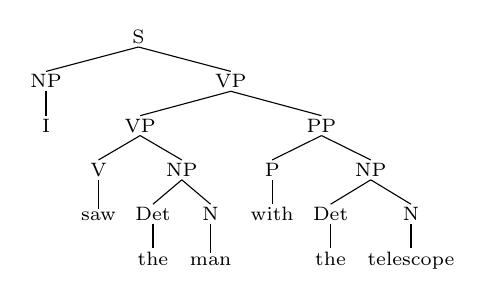
\begin{tikzpicture}[level distance=16pt,sibling distance=5pt,
        every node/.style={font=\scriptsize,inner sep=1pt}]
      \Tree [.S [.NP I ] [.VP [.VP [.V saw ] [.NP [.Det the ] [.N man ] ] ]
        [.PP [.P with ] [.NP [.Det the ] [.N telescope ] ] ] ] ]
    \end{tikzpicture}
    \par\smallskip
    The PP modifies the seeing event:\\I used the telescope.
    \column{0.49\textwidth}
    \centering
    \textbf{B: PP attaches to NP}\\[3pt]
    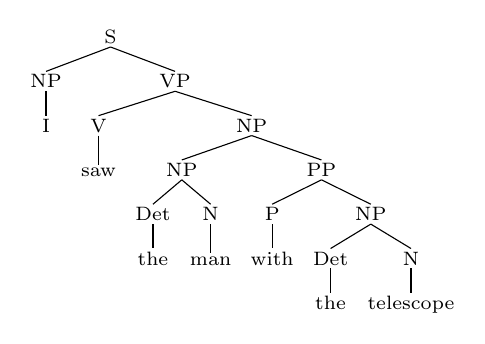
\begin{tikzpicture}[level distance=16pt,sibling distance=5pt,
        every node/.style={font=\scriptsize,inner sep=1pt}]
      \Tree [.S [.NP I ] [.VP [.V saw ] [.NP [.NP [.Det the ] [.N man ] ]
        [.PP [.P with ] [.NP [.Det the ] [.N telescope ] ] ] ] ] ]
    \end{tikzpicture}
    \par\smallskip
    The PP modifies the object:\\the man had the telescope.
  \end{columns}
  \pause
  \begin{block}{Bridge to the dangling else}
    Later, an \texttt{else} can attach to an inner or outer \texttt{if}.
    Both ask: \emph{which constituent receives this attachment?}
    The telescope example is PP attachment, not a dangling modifier.
  \end{block}
\end{frame}

\begin{frame}{Coordination Ambiguity: Is Dessert Always Included?}
  \small
  A restaurant advertises: \textbf{``Free soup or salad and dessert.''}
  Focus on the grouping of \emph{soup or salad and dessert}; treat
  \emph{or} as a choice and \emph{and} as a bundle for this example.
  \[
    M\to M\ \text{or}\ M\mid M\ \text{and}\ M
      \mid\text{soup}\mid\text{salad}\mid\text{dessert}.
  \]
  \begin{columns}[T]
    \column{0.49\textwidth}
    \begin{block}{A: soup or (salad and dessert)}
      \centering
      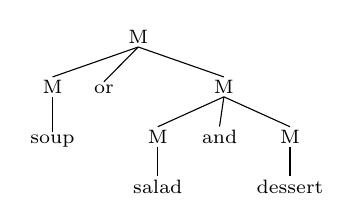
\begin{tikzpicture}[level distance=18pt,sibling distance=5pt,
          every node/.style={font=\scriptsize,inner sep=1pt}]
        \Tree [.M [.M soup ] or [.M [.M salad ] and [.M dessert ] ] ]
      \end{tikzpicture}
      \par\smallskip
      Dessert comes only with salad.\\
      \emph{And} groups more tightly here.
    \end{block}
    \column{0.49\textwidth}
    \begin{block}{B: (soup or salad) and dessert}
      \centering
      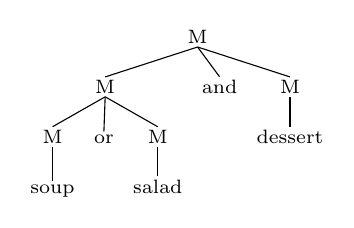
\begin{tikzpicture}[level distance=18pt,sibling distance=5pt,
          every node/.style={font=\scriptsize,inner sep=1pt}]
        \Tree [.M [.M [.M soup ] or [.M salad ] ] and [.M dessert ] ]
      \end{tikzpicture}
      \par\smallskip
      Dessert comes with either choice.\\
      \emph{Or} groups more tightly here.
    \end{block}
  \end{columns}
  \pause
  This is the same grouping issue as $5+3\times2$:
  $(5+3)\times2=16$, while $5+(3\times2)=11$.
  The usual arithmetic convention selects $11$; an ambiguous grammar alone
  does not enforce that convention. The next slides encode it explicitly.
\end{frame}

\begin{frame}{Ambiguous Arithmetic Grammar}
  Consider
  \[
    E\to E+E\mid E\times E\mid\mathrm{id}.
  \]
  The string $\mathrm{id}+\mathrm{id}\times\mathrm{id}$ has two structures:
  \begin{columns}[T]
    \column{0.49\textwidth}
    \centering $(\mathrm{id}+\mathrm{id})\times\mathrm{id}$
    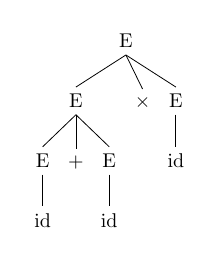
\begin{tikzpicture}[scale=0.72]
      \Tree [.E [.E [.E $\mathrm{id}$ ] + [.E $\mathrm{id}$ ] ] $\times$ [.E $\mathrm{id}$ ] ]
    \end{tikzpicture}

    \column{0.49\textwidth}
    \centering $\mathrm{id}+(\mathrm{id}\times\mathrm{id})$
    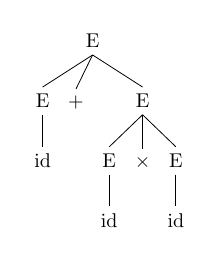
\begin{tikzpicture}[scale=0.72]
      \Tree [.E [.E $\mathrm{id}$ ] + [.E [.E $\mathrm{id}$ ] $\times$ [.E $\mathrm{id}$ ] ] ]
    \end{tikzpicture}
  \end{columns}
  The grammar does not encode precedence or associativity.
\end{frame}

\begin{frame}{The Same Ambiguity as Leftmost Derivations}
  For $\mathrm{id}+\mathrm{id}\times\mathrm{id}$:
  \begin{block}{Top-level multiplication}
    \begin{align*}
      E&\Rightarrow_{\mathrm{lm}}E\times E
       \Rightarrow_{\mathrm{lm}}E+E\times E
       \Rightarrow_{\mathrm{lm}}\mathrm{id}+E\times E\\
       &\Rightarrow_{\mathrm{lm}}\mathrm{id}+\mathrm{id}\times E
       \Rightarrow_{\mathrm{lm}}\mathrm{id}+\mathrm{id}\times\mathrm{id}.
    \end{align*}
  \end{block}
  \begin{block}{Top-level addition}
    \begin{align*}
      E&\Rightarrow_{\mathrm{lm}}E+E
       \Rightarrow_{\mathrm{lm}}\mathrm{id}+E
       \Rightarrow_{\mathrm{lm}}\mathrm{id}+E\times E\\
       &\Rightarrow_{\mathrm{lm}}\mathrm{id}+\mathrm{id}\times E
       \Rightarrow_{\mathrm{lm}}\mathrm{id}+\mathrm{id}\times\mathrm{id}.
    \end{align*}
  \end{block}
\end{frame}

\begin{frame}{Encoding Precedence and Associativity}
  Replace the ambiguous grammar by
  \[
    \begin{aligned}
      E&\to E+T\mid T,\\
      T&\to T\times F\mid F,\\
      F&\to(E)\mid\mathrm{id}.
    \end{aligned}
  \]
  \begin{itemize}
    \item Multiplication binds more tightly because it is formed inside $T$ before $T$ participates in addition.
    \item Left recursion in $E\to E+T$ makes addition left-associative.
    \item Left recursion in $T\to T\times F$ makes multiplication left-associative.
    \item Parentheses allow a factor to contain an entire expression.
  \end{itemize}
  For right-associative addition, one could instead use $E\to T+E\mid T$.
\end{frame}

\begin{frame}{The Dangling-Else Ambiguity}
  \small
  Like the telescope's PP, the \texttt{else} has two possible attachment sites.
  The natural grammar
  \[
    S\to \mathbf{if}\ c\ \mathbf{then}\ S
      \mid \mathbf{if}\ c\ \mathbf{then}\ S\ \mathbf{else}\ S
      \mid a
  \]
  where $c$ stands for a condition and $a$ for any other statement. The grammar
  is ambiguous: in
  \[
    \mathbf{if}\ c\ \mathbf{then}\
    \mathbf{if}\ c\ \mathbf{then}\ a\ \mathbf{else}\ a,
  \]
  the $\mathbf{else}$ may attach to either $\mathbf{if}$.
  \begin{block}{Standard matched/unmatched solution}
    \[
      \begin{aligned}
        S&\to M\mid U,\\
        M&\to a\mid \mathbf{if}\ c\ \mathbf{then}\ M\ \mathbf{else}\ M,\\
        U&\to \mathbf{if}\ c\ \mathbf{then}\ S
          \mid \mathbf{if}\ c\ \mathbf{then}\ M\ \mathbf{else}\ U.
      \end{aligned}
    \]
  \end{block}
  This grammar attaches each $\mathbf{else}$ to the nearest unmatched $\mathbf{if}$.
\end{frame}

\begin{frame}{Grammar Ambiguity Versus Inherent Ambiguity}
  \begin{itemize}
    \item A \textbf{grammar} is ambiguous when it gives some string two parse trees.
    \item A \textbf{language} is inherently ambiguous when every CFG generating it is ambiguous.
  \end{itemize}
  An ambiguous grammar may still describe a language that has another unambiguous grammar; arithmetic
  expressions are an example.
  \begin{block}{Standard inherently ambiguous language}
    \[
      \{a^i b^j c^k\mid i=j\text{ or }j=k,\ i,j,k\ge1\}.
    \]
  \end{block}
  \begin{alertblock}{Algorithmic limitation}
    There is no general algorithm that decides whether an arbitrary CFG is ambiguous.
  \end{alertblock}
\end{frame}

\begin{frame}{Understanding an Inherently Ambiguous Language}
  \small
  Write the standard example as a union:
  \[
    \begin{aligned}
      L_{ab}&=\{a^n b^n c^k:n,k\ge1\},\\
      L_{bc}&=\{a^i b^n c^n:i,n\ge1\},\\
      L&=L_{ab}\cup L_{bc}.
    \end{aligned}
  \]
  \begin{columns}[T]
    \column{0.43\textwidth}
    \centering
    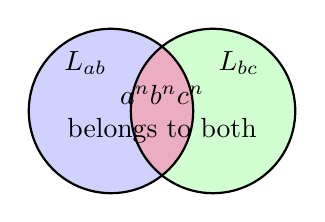
\begin{tikzpicture}[scale=0.72]
      % Fill both sets, then explicitly repaint their lens-shaped intersection.
      % This avoids the second circle visually covering the first set's share
      % of the overlap in PDF renderers without transparency blending.
      \fill[blue!18] (-0.9,0) circle (1.45);
      \fill[green!18] (0.9,0) circle (1.45);
      \begin{scope}
        \clip (-0.9,0) circle (1.45);
        \fill[purple!32] (0.9,0) circle (1.45);
      \end{scope}
      \draw[thick] (-0.9,0) circle (1.45);
      \draw[thick] (0.9,0) circle (1.45);
      \node at (-1.35,0.85) {$L_{ab}$};
      \node at (1.35,0.85) {$L_{bc}$};
      \node[align=center] at (0,-0.05)
        {$a^n b^n c^n$\\belongs to both};
    \end{tikzpicture}
    \column{0.54\textwidth}
    Strings $a^n b^n c^n$ have two natural structural explanations:
    \begin{itemize}
      \item match the $a$- and $b$-counts using $L_{ab}$; or
      \item match the $b$- and $c$-counts using $L_{bc}$.
    \end{itemize}
    A direct union grammar therefore gives such strings two parse trees.
  \end{columns}
  \begin{alertblock}{Why the theorem is stronger}
    Two parses in one convenient grammar prove only that grammar ambiguous.
    The inherent-ambiguity theorem proves that \emph{every} CFG for $L$ must
    be ambiguous; no grammar refactoring or normal-form conversion can remove
    the conflict. The proof that this is unavoidable is substantially deeper
    than displaying the two natural parses.
  \end{alertblock}
\end{frame}

% ==========================================
% Part 5: Simple (s-) Grammars
% ==========================================
\section{Simple Grammars (s-Grammars)}

\begin{frame}{Definition of an $s$-Grammar}
  \small
  \begin{block}{Simple grammar (Linz)}
    A CFG is an \textbf{$s$-grammar} if every production has the form
    \[
      A\to a\alpha,
    \]
    where $A\in V$, $a\in T$, and $\alpha\in V^*$, and for each pair
    $(A,a)$ there is at most one such production.
  \end{block}
  Thus every right-hand side begins with a terminal, followed by zero or more
  variables. The uniqueness condition means that the current variable and the
  next input symbol determine at most one production.
  \pause
  \begin{alertblock}{Standard convention}
    The basic definition has no $\varepsilon$-productions, so an
    $s$-grammar does not generate $\varepsilon$. Some presentations add a
    separately controlled start rule for the empty word.
  \end{alertblock}
\end{frame}

\begin{frame}{Worked $s$-Grammar Example}
  \small
  Consider
  \[
    S\to aAB\mid bB,\qquad
    A\to aA\mid b,\qquad
    B\to b.
  \]
  Every production begins with a terminal, and no variable has two
  productions beginning with the same terminal. Hence this is an $s$-grammar.
  \begin{exampleblock}{Leftmost derivation of $aabb$}
    \[
      S\Rightarrow aAB
       \Rightarrow aaAB
       \Rightarrow aabB
       \Rightarrow aabb.
    \]
  \end{exampleblock}
  At each step the next unmatched input symbol uniquely determines the
  production: $(S,a)$ selects $S\to aAB$, $(A,a)$ selects $A\to aA$,
  $(A,b)$ selects $A\to b$, and $(B,b)$ selects $B\to b$.
\end{frame}

\begin{frame}{Predictive Recognition for an $s$-Grammar}
  \small
  A simple top-down recognizer stores the unexpanded variables, with the next
  variable at the left of the stack.
  \begin{center}
  \begin{tabular}{L{2.2cm}L{2.7cm}L{5.4cm}}
    \toprule
    Input remaining & Variable stack & Action for the example grammar \\
    \midrule
    $aabb$ & $S$ & use $S\to aAB$; match $a$ \\
    $abb$ & $AB$ & use $A\to aA$; match $a$ \\
    $bb$ & $AB$ & use $A\to b$; match $b$ \\
    $b$ & $B$ & use $B\to b$; match $b$ \\
    $\varepsilon$ & $\varepsilon$ & accept \\
    \bottomrule
  \end{tabular}
  \end{center}
  \begin{block}{Consequences}
    The production choice never requires backtracking. Therefore every
    $s$-grammar is unambiguous, although many unambiguous CFLs cannot be
    generated by an $s$-grammar.
  \end{block}
\end{frame}

\begin{frame}{What Fails the $s$-Grammar Test?}
  \small
  \begin{columns}[T]
    \column{0.48\textwidth}
    \begin{exampleblock}{Valid}
      \[
        S\to aA\mid bB,\qquad
        A\to a\mid bA.
      \]
      For $S$, the leading terminals are distinct; the same is true for $A$.
    \end{exampleblock}
    \column{0.48\textwidth}
    \begin{alertblock}{Not simple}
      \[
        S\to aA\mid aB,\qquad
        A\to b,\quad B\to c.
      \]
      The pair $(S,a)$ occurs twice, so lookahead $a$ does not choose a unique
      production.
    \end{alertblock}
  \end{columns}
  \vspace{0.2cm}
  Rules such as $S\to AB$, $S\to\varepsilon$, or $S\to abA$ also violate the
  basic form: the first begins with a variable, the second has no leading
  terminal, and the third has a terminal after its first position.
\end{frame}

% ==========================================
% Part 6: Normal Forms
% ==========================================
\section{Normal Forms for CFGs}

\begin{frame}{Why Put a CFG in Normal Form?}
  \small
  A normal form restricts the shapes of productions without changing the
  generated language. The restricted structure makes proofs and algorithms
  easier to state and analyze.
  \begin{block}{Two standard forms}
    \begin{itemize}
      \item \textbf{Chomsky normal form (CNF):} parse trees are binary, which
        supports CYK parsing and the standard pumping-lemma proof.
      \item \textbf{Greibach normal form (GNF):} every production emits a
        terminal first, closely connecting leftmost derivations with input
        consumption by a pushdown automaton.
    \end{itemize}
  \end{block}
  \pause
  \begin{alertblock}{Language equivalence, not identical grammar behavior}
    Conversion preserves the language (with a controlled exception for
    $\varepsilon$), but may change parse-tree shape, derivation length, and
    ambiguity behavior.
  \end{alertblock}
\end{frame}

\begin{frame}{Meaning of Equivalent Normal Form}
  \small
  \begin{block}{Weak or language equivalence}
    Grammars $G$ and $G'$ are equivalent for this course when
    \[
      L(G)=L(G').
    \]
    CNF and GNF conversion guarantee this equality, subject to the explicit
    convention used for $\varepsilon$.
  \end{block}
  They do \emph{not} generally preserve:
  \begin{itemize}
    \item the names or number of variables and productions;
    \item the exact derivation sequence or shape of the parse tree;
    \item the number of derivations associated with a word; or
    \item a convenient mapping to an intended abstract syntax tree.
  \end{itemize}
  \begin{alertblock}{Can every CFG be converted?}
    Every context-free language has a CNF grammar and a GNF grammar. If
    $\varepsilon$ belongs to the language, both forms use the standard
    exceptional start rule $S_0\to\varepsilon$, with $S_0$ absent from all
    right-hand sides.
  \end{alertblock}
\end{frame}

\begin{frame}{The Empty String Requires Special Treatment}
  \small
  The rule $A\to\varepsilon$ can erase a variable inside a larger sentential
  form. This complicates binary parse-tree arguments and algorithms whose
  table cells represent \emph{nonempty} input spans.
  \pause
  \begin{block}{Standard segregation approach}
    Separate the empty word from the nonempty part of the language:
    \[
      L=L^+\cup
      \begin{cases}
        \{\varepsilon\},&\varepsilon\in L,\\
        \varnothing,&\varepsilon\notin L,
      \end{cases}
      \qquad L^+=L\setminus\{\varepsilon\}.
    \]
    Introduce a fresh start variable $S_0$ that never occurs on a right-hand
    side. Preserve $S_0\to\varepsilon$ when necessary, then eliminate every
    other null production.
  \end{block}
  \pause
  \begin{exampleblock}{Example}
    For $S\to aSb\mid\varepsilon$, use
    \[
      S_0\to S\mid\varepsilon,
      \qquad
      S\to aSb\mid ab.
    \]
    The second line generates the nonempty words; the exceptional start rule
    handles $\varepsilon$. A later unit-production step removes $S_0\to S$.
  \end{exampleblock}
  CYK likewise handles an empty input by a separate test for
  $S_0\to\varepsilon$.
\end{frame}

\begin{frame}{Eliminating Null Productions}
  \small
  A \textbf{null production} is a rule $A\to\varepsilon$. A variable is
  \textbf{nullable} if it derives $\varepsilon$ in zero or more steps.
  \pause
  \begin{block}{Procedure}
    \begin{enumerate}
      \item Mark every $A$ for which $A\to\varepsilon$ is a production.
      \item Repeatedly mark $A$ when some rule
        $A\to X_1\cdots X_k$ has every $X_i$ already marked nullable.
      \item For each production, add every nonempty alternative obtained by
        deleting any subset of its nullable-variable occurrences.
      \item Remove the original null productions.
      \item If $\varepsilon\in L(G)$ must be preserved, introduce a fresh
        start variable $S_0$ and retain $S_0\to\varepsilon$.
    \end{enumerate}
  \end{block}
  Different subsets can produce the same rule; duplicate productions are kept
  only once.
\end{frame}

\begin{frame}{Worked Null-Production Elimination}
  \small
  Consider
  \[
    S\to AB\mid a,\qquad
    A\to aA\mid\varepsilon,\qquad
    B\to bB\mid\varepsilon.
  \]
  Variables $A$ and $B$ are nullable directly, and $S$ is nullable through
  $S\Rightarrow AB\Rightarrow^*\varepsilon$.
  \begin{block}{Grammar after null elimination}
    \[
      \begin{aligned}
        S_0&\to S\mid\varepsilon,\\
        S&\to AB\mid A\mid B\mid a,\\
        A&\to aA\mid a,\\
        B&\to bB\mid b.
      \end{aligned}
    \]
  \end{block}
  From $S\to AB$, deleting nullable occurrences gives $S\to A$, $S\to B$,
  and $S\to\varepsilon$; the last alternative is represented only by the
  fresh start rule. Similarly, $A\to aA$ yields $A\to a$ and
  $B\to bB$ yields $B\to b$.
\end{frame}

\begin{frame}{Eliminating Unit Productions}
  \small
  A \textbf{unit production} has the form $A\to B$, with both sides variables.
  \begin{block}{Procedure}
    \begin{enumerate}
      \item Compute all \textbf{unit pairs} $(A,B)$ such that
        $A\Rightarrow^* B$ using only unit productions.
      \item For every unit pair $(A,B)$, copy each non-unit production
        $B\to\alpha$ to $A\to\alpha$.
      \item Delete all unit productions and remove duplicates.
    \end{enumerate}
  \end{block}
  \begin{exampleblock}{Example}
    From
    \[
      S\to A\mid b,\quad A\to B\mid a,\quad B\to bB\mid c,
    \]
    the unit pairs include $(S,A)$, $(S,B)$, and $(A,B)$. The equivalent
    unit-free rules are
    \[
      S\to b\mid a\mid bB\mid c,\quad
      A\to a\mid bB\mid c,\quad
      B\to bB\mid c.
    \]
  \end{exampleblock}
\end{frame}

\begin{frame}{Removing Useless Productions and Symbols}
  \small
  A variable is useful only if it can derive a terminal word and can occur in
  some derivation from the start variable.
  \begin{block}{Two-pass procedure}
    \begin{enumerate}
      \item \textbf{Generating pass:} Mark variables with a terminal-only
        production, then repeatedly mark $A$ if some $A\to\alpha$ contains
        only terminals and already generating variables. Remove everything
        involving an unmarked variable.
      \item \textbf{Reachability pass:} Mark $S$. Whenever a marked variable
        has a production containing variable $B$, mark $B$. Remove all
        remaining unmarked variables and their productions.
    \end{enumerate}
  \end{block}
  For
  \[
    S\to AB\mid a,\quad A\to aA\mid a,\quad B\to b,\quad
    C\to cC\mid c,\quad D\to dD,
  \]
  $D$ is non-generating and is removed first; $C$ is generating but
  unreachable and is removed in the second pass. Only $S,A,B$ remain.
\end{frame}

\begin{frame}{Chomsky Normal Form (CNF)}
  \small
  \begin{block}{Definition}
    A CFG is in Chomsky normal form when every production has one of the forms
    \[
      A\to BC
      \qquad\text{or}\qquad
      A\to a,
    \]
    where $A,B,C$ are variables and $a$ is a terminal. If
    $\varepsilon\in L(G)$, the additional rule $S_0\to\varepsilon$ is allowed,
    provided the start variable $S_0$ never occurs on a right-hand side.
  \end{block}
  \pause
  \begin{itemize}
    \item Unit rules $A\to B$, mixed rules $A\to aB$, and right-hand sides of
      length greater than two are not in CNF.
    \item Every CFL has an equivalent CNF grammar under the start-symbol
      convention above.
    \item A nonempty word of length $n$ has a binary CNF parse tree with
      exactly $n$ terminal leaves.
  \end{itemize}
\end{frame}

\begin{frame}{A Reliable CNF Conversion Pipeline}
  \small
  Given $G=(V,T,S,P)$, apply the following language-preserving steps:
  \begin{enumerate}
    \item Introduce a fresh start variable $S_0$ with $S_0\to S$.
    \item Eliminate $\varepsilon$-productions, retaining
      $S_0\to\varepsilon$ only when $\varepsilon\in L(G)$.
    \item Eliminate unit productions such as $A\to B$.
    \item Remove useless variables that are non-generating or unreachable.
    \item In a right-hand side of length at least two, replace each terminal
      $a$ by a variable $A_a$ with $A_a\to a$.
    \item Binarize every long rule. For example,
      $A\to BCD$ becomes $A\to BX$ and $X\to CD$.
  \end{enumerate}
  \pause
  \begin{alertblock}{Order matters}
    Removing $\varepsilon$- and unit productions can create new short rules,
    so perform those simplifications before terminal replacement and
    binarization.
  \end{alertblock}
\end{frame}

\begin{frame}{Worked CNF Conversion}
  \small
  Convert the grammar
  \[
    S\to aSb\mid ab,
  \]
  which generates $\{a^n b^n:n\ge1\}$.
  \begin{enumerate}
    \item Introduce variables for terminals used in longer productions:
      \[
        A\to a,\qquad B\to b.
      \]
    \item Replace the terminal occurrences:
      \[
        S\to ASB\mid AB.
      \]
    \item Binarize the length-three rule using $X\to SB$:
      \[
        \boxed{S\to AX\mid AB,\quad X\to SB,\quad A\to a,\quad B\to b.}
      \]
  \end{enumerate}
  Every rule is now of the form variable-to-two-variables or
  variable-to-one-terminal. For example,
  $S\Rightarrow AX\Rightarrow aX\Rightarrow aSB\Rightarrow aABB
  \Rightarrow aaBB\Rightarrow aabB\Rightarrow aabb$.
\end{frame}

\begin{frame}{CYK Parsing: Dynamic-Programming Table}
  \small
  The Cocke--Younger--Kasami (CYK) algorithm decides membership for a grammar
  in CNF. For input $w=a_1a_2\cdots a_n$, define
  \[
    T[i,\ell]
    =\{A\in V:A\Rightarrow^*a_i\cdots a_{i+\ell-1}\}.
  \]
  Thus $T[i,\ell]$ contains the variables that generate the substring of
  length $\ell$ beginning at position $i$.
  \pause
  \begin{block}{Recurrence}
    \begin{align*}
      T[i,1]
        &=\{A:A\to a_i\in P\},\\
      T[i,\ell]
        &=\bigcup_{k=1}^{\ell-1}
          \{A:A\to BC,\ B\in T[i,k],\
          C\in T[i+k,\ell-k]\}.
    \end{align*}
  \end{block}
  Fill the table from shorter substrings to longer substrings. The algorithm
  accepts exactly when
  \[
    S\in T[1,n].
  \]
  If the grammar permits $S\to\varepsilon$, test the empty input separately.
\end{frame}

\begin{frame}{CYK Algorithm and Complexity}
  \small
  \begin{block}{Bottom-up procedure}
    \begin{enumerate}
      \item Initialize every length-one cell using terminal rules $A\to a_i$.
      \item For lengths $\ell=2,\ldots,n$, examine every starting position $i$.
      \item Try every split $k$ of the substring into lengths $k$ and
        $\ell-k$.
      \item For each binary rule $A\to BC$, insert $A$ when the left cell
        contains $B$ and the right cell contains $C$.
      \item Accept iff the start variable occurs in the top cell.
    \end{enumerate}
  \end{block}
  \pause
  Let $P_2$ be the set of binary productions.
  \[
    \boxed{\text{Time }O(n^3|P_2|),\qquad
           \text{space }O(n^2|V|).}
  \]
  For a fixed grammar, this is conventionally reported as $O(n^3)$ time and
  $O(n^2)$ table space. CNF conversion is preprocessing and its cost is
  separate from parsing a particular input word.
\end{frame}

\begin{frame}{Worked CYK Example: Parsing $aabb$}
  \small
  Use the CNF grammar from the preceding conversion:
  \[
    S\to AX\mid AB,\qquad X\to SB,\qquad A\to a,\qquad B\to b.
  \]
  \begin{center}
  \renewcommand{\arraystretch}{1.25}
  \begin{tabular}{c|cccc}
    \toprule
    Substring length & Start 1 & Start 2 & Start 3 & Start 4\\
    \midrule
    $1$ & $\{A\}$ & $\{A\}$ & $\{B\}$ & $\{B\}$\\
    $2$ & $\varnothing$ & $\{S\}$ & $\varnothing$ & ---\\
    $3$ & $\varnothing$ & $\{X\}$ & --- & ---\\
    $4$ & $\{S\}$ & --- & --- & ---\\
    \bottomrule
  \end{tabular}
  \end{center}
  For example, $T[2,2]=\{S\}$ because the substring $ab$ splits into
  $\{A\}\{B\}$ and $S\to AB$. Then $T[2,3]=\{X\}$ because
  $X\to SB$, and finally $T[1,4]=\{S\}$ because $S\to AX$.
  \begin{exampleblock}{Decision}
    Since $S\in T[1,4]$, CYK accepts $aabb$.
  \end{exampleblock}
\end{frame}

\begin{frame}{Important CKY/CYK Extensions}
  \small
  The names \textbf{CYK} and \textbf{CKY} denote the same core dynamic
  program; CKY is especially common in computational linguistics.
  \pause
  \begin{center}
  \begin{tabular}{L{3.0cm}L{7.4cm}}
    \toprule
    Extension & Significant distinction \\
    \midrule
    \paperlink{https://web.stanford.edu/\string~jurafsky/slp3/19.pdf}
      {Backpointer CKY} & Stores successful split points and child variables,
      reconstructing a parse tree rather than answering membership only. \\
    \paperlink{https://aclanthology.org/P89-1018/}
      {Packed-forest CKY} & Shares common subtrees so that many parses of an
      ambiguous sentence can be represented compactly. \\
    \paperlink{https://web.stanford.edu/\string~jurafsky/slp3/old_jan23/C.pdf}
      {Viterbi CKY} & For a probabilistic CFG, replaces Boolean values by maximum
      probabilities and returns the highest-probability parse. \\
    \paperlink{https://aclanthology.org/W16-5901/}
      {Inside--outside CKY} & Sums probabilities of all parses; the outside pass
      supports marginal probabilities and PCFG estimation. \\
    \paperlink{https://doi.org/10.1016/S0022-0000(75)80046-8}
      {Valiant's algorithm} & Reformulates general CFG recognition using Boolean
      matrix multiplication, giving a theoretically subcubic alternative to
      the standard cubic recurrence. \\
    \bottomrule
  \end{tabular}
  \end{center}
\end{frame}

\begin{frame}{CYK in Practice and Important Alternatives}
  \footnotesize
  \textbf{Real-world connection.}
  In natural-language processing, probabilistic CKY ranks competing
  constituency analyses using a PCFG, while a packed chart shares repeated
  subtrees.
  \begin{center}
  \begin{tabular}{L{2.5cm}L{3.0cm}L{4.8cm}}
    \toprule
    Method & Grammar requirement & Main distinction \\
    \midrule
    \paperlink{https://web.stanford.edu/\string~jurafsky/slp3/19.pdf}
      {CYK/CKY} & CNF or binarized CFG & Simple span dynamic programming;
      cubic worst-case time. \\
    \paperlink{https://doi.org/10.1145/362007.362035}
      {Earley parser} & Arbitrary CFG & Prediction, scanning, and completion;
      no CNF conversion and cubic worst case. \\
    \paperlink{https://aclanthology.org/J87-1004/}
      {GLR/Tomita} & Generalized LR treatment & Uses a graph-structured stack to
      pursue conflicts and represent ambiguous parses. \\
    \paperlink{https://doi.org/10.1016/S0019-9958(65)90426-2}
      {LL/LR parsers} & Restricted deterministic CFGs & Typically linear-time
      parsing; dominant for programming-language syntax. \\
    \bottomrule
  \end{tabular}
  \end{center}
  \textbf{Terminology:} Earley, GLR, and LL/LR are alternatives, not variants
  of the CYK recurrence; their grammar requirements and engineering goals
  differ. Blue method names link to the core paper or a standard resource.
\end{frame}

\begin{frame}{Greibach Normal Form (GNF)}
  \small
  \begin{block}{Definition}
    A CFG is in Greibach normal form when every production has the form
    \[
      A\to aA_1A_2\cdots A_k,
      \qquad k\ge0,
    \]
    where $a$ is a terminal and each $A_i$ is a variable. As in CNF, a fresh
    start rule $S_0\to\varepsilon$ may be allowed when the language contains
    $\varepsilon$.
  \end{block}
  \pause
  \begin{itemize}
    \item Every non-$\varepsilon$ production begins with exactly one terminal.
    \item Each step of a leftmost derivation produces exactly one new terminal;
      hence a word of length $n$ is derived in exactly $n$ steps.
    \item Every CFL has an equivalent GNF grammar, subject to the usual
      treatment of $\varepsilon$.
  \end{itemize}
\end{frame}

\begin{frame}{A Systematic GNF Conversion Outline}
  \small
  A full GNF construction is more involved than CNF conversion. A standard
  outline is:
  \begin{enumerate}
    \item Introduce a fresh start variable and remove null, unit, and useless
      productions.
    \item Replace terminals occurring after the first position by helper
      variables, such as $B_b\to b$.
    \item Order the variables $A_1,\ldots,A_n$.
    \item Whenever a rule for $A_i$ begins with $A_j$ for $j<i$, substitute
      the productions of $A_j$. Eliminate any immediate left recursion thereby
      exposed.
    \item Process variables in reverse order, repeatedly substituting a
      leading variable until every right-hand side begins with a terminal.
    \item Put any helper variables introduced during left-recursion removal
      into the same terminal-leading form.
  \end{enumerate}
  \begin{alertblock}{Practical perspective}
    The construction proves expressive equivalence but may increase grammar
    size substantially. Production parsers usually target LL/LR-style
    grammars directly rather than converting a programming-language grammar
    to GNF.
  \end{alertblock}
\end{frame}

\begin{frame}{Worked GNF Conversion: Removing Left Recursion}
  \small
  The grammar
  \[
    S\to Sa\mid b
  \]
  generates $ba^*$, but is not in GNF: one rule begins with a variable and it
  is immediately left-recursive.
  \begin{block}{Equivalent GNF grammar}
    \[
      \boxed{S\to b\mid bA,\qquad A\to a\mid aA.}
    \]
  \end{block}
  Every production begins with a terminal followed only by variables. The
  derivation
  \[
    S\Rightarrow bA\Rightarrow baA\Rightarrow baa
  \]
  generates $baa$. In general, $S\to b$ produces zero $a$'s, while
  $S\to bA$ followed by the rules for $A$ produces one or more $a$'s.
  \begin{alertblock}{Typical GNF strategy}
    Order variables, substitute productions that begin with earlier variables,
    eliminate left recursion, and continue until every rule begins with a
    terminal.
  \end{alertblock}
\end{frame}

\begin{frame}{Do Normal Forms Remove Ambiguity?}
  \small
  \begin{alertblock}{No}
    CNF and GNF constrain production shape; they do not guarantee a unique
    parse tree.
  \end{alertblock}
  \pause
  \begin{columns}[T]
    \column{0.47\textwidth}
    \begin{block}{Ambiguous CNF grammar}
      \[
        S\to SS\mid a.
      \]
      The word $aaa$ has the groupings $(aa)a$ and $a(aa)$, so a grammar can
      be both CNF and ambiguous.
    \end{block}
    \column{0.47\textwidth}
    \begin{block}{Ambiguous GNF grammar}
      \[
        S\to aS\mid aA\mid a,\qquad A\to a.
      \]
      The word $aa$ has derivations $S\Rightarrow aS\Rightarrow aa$ and
      $S\Rightarrow aA\Rightarrow aa$.
    \end{block}
  \end{columns}
  \begin{itemize}
    \item If a language is inherently ambiguous, every equivalent normal-form
      grammar remains ambiguous.
    \item If only the original grammar is ambiguous, ambiguity must be handled
      by grammar redesign or explicit disambiguation rules—not merely by
      normal-form conversion.
  \end{itemize}
\end{frame}

\begin{frame}{GNF Versus an $s$-Grammar}
  \small
  \begin{center}
  \begin{tabular}{L{3.1cm}L{7.0cm}}
    \toprule
    Form & Restriction \\
    \midrule
    GNF & Every production is $A\to a\alpha$, where $a\in T$ and
      $\alpha\in V^*$. \\
    $s$-grammar & It is in GNF, and for each pair $(A,a)$ there is at most one
      production whose left side is $A$ and whose first terminal is $a$. \\
    \bottomrule
  \end{tabular}
  \end{center}
  \begin{columns}[T]
    \column{0.49\textwidth}
    \begin{exampleblock}{$s$-grammar}
      \[
        \begin{aligned}
          S&\to aA\mid bB,\\
          A&\to aA\mid b,\\
          B&\to bB\mid a.
        \end{aligned}
      \]
      The next terminal uniquely selects a rule for the current variable.
    \end{exampleblock}
    \column{0.49\textwidth}
    \begin{alertblock}{GNF, but not an $s$-grammar}
      \[
        \begin{aligned}
          S&\to aA\mid aB,\\
          A&\to b,\qquad B\to c.
        \end{aligned}
      \]
      Both productions for $S$ begin with $a$, violating uniqueness.
    \end{alertblock}
  \end{columns}
\end{frame}

\begin{frame}{Other Useful Grammar Forms and Restrictions}
  \small
  CNF and GNF are the principal universal normal forms for CFGs, but related
  forms are useful in specialized settings.
  \begin{center}
  \begin{tabular}{L{3.2cm}L{7.1cm}}
    \toprule
    Form or restriction & Main purpose and limitation \\
    \midrule
    Reduced/proper grammar & Removes useless, null, and unit productions;
      commonly used as preprocessing. \\
    Binary or 2-normal form & Bounds right-hand-side length by two but may
      allow mixtures such as $A\to aB$; weaker than CNF. \\
    Operator form & Avoids adjacent variables and supports
      operator-precedence techniques for expression-like grammars; not a
      universal deterministic parsing solution. \\
    LL($k$), LR($k$) restrictions & Enable efficient deterministic parsing,
      often linear in input length, but not every CFL has such a grammar. \\
    Kuroda normal form & A normal form for context-sensitive grammars, not a
      CFG normal form. \\
    \bottomrule
  \end{tabular}
  \end{center}
  These forms answer different questions: descriptive equivalence, proof
  convenience, or efficient deterministic parsing.
\end{frame}

% ==========================================
% Part 7: Properties of CFLs
% ==========================================
\section{Properties of Context-Free Languages}

\begin{frame}{Closure Properties of CFLs}
  \small
  Context-free languages are closed under several constructive operations.
  If $L_1$ and $L_2$ are CFLs, then the following are CFLs:
  \begin{itemize}
    \item $L_1\cup L_2$ (union), $L_1L_2$ (concatenation), and $L_1^*$ (Kleene star);
    \item $L_1^R$ (reversal);
    \item $h(L_1)$ for a homomorphism $h$;
    \item $h^{-1}(L_1)$ for an inverse homomorphism; and
    \item $L_1\cap R$ and $L_1\setminus R$ when $R$ is regular.
  \end{itemize}
  \pause
  \begin{alertblock}{Not all regular-language properties carry over}
    CFLs are not closed under intersection, complement, or difference of two arbitrary CFLs.
  \end{alertblock}
\end{frame}

\begin{frame}{Closure by Grammar Construction}
  Let $G_1$ and $G_2$ have disjoint variable sets and start variables $S_1,S_2$.
  Introduce a fresh start variable $S$.
  \begin{center}
  \begin{tabular}{L{2.7cm}L{3.8cm}L{3.7cm}}
    \toprule
    Language & New productions & Why it works \\
    \midrule
    $L_1\cup L_2$ & $S\to S_1\mid S_2$ & choose either grammar \\
    $L_1L_2$ & $S\to S_1S_2$ & generate one word from each \\
    $L_1^*$ & $S\to S_1S\mid\varepsilon$ & generate zero or more factors \\
    \bottomrule
  \end{tabular}
  \end{center}
  \begin{block}{Reversal}
    Reverse the right-hand side of every production. Reversing each local child order reverses the
    yield of every parse tree, so the new grammar generates $L_1^R$.
  \end{block}
\end{frame}

\begin{frame}{Worked Closure Examples}
  \small
  Let
  \[
    L_1=\{a^n b^n:n\ge0\},
    \qquad
    L_2=\{a^n c^n:n\ge0\}.
  \]
  Grammars $A\to aAb\mid\varepsilon$ and
  $B\to aBc\mid\varepsilon$ generate $L_1$ and $L_2$.

  \begin{block}{Union and concatenation}
    \begin{align*}
      S_U&\to A\mid B
        &&\text{generates }L_1\cup L_2,\\
      S_C&\to AB
        &&\text{generates }L_1L_2
          =\{a^i b^i a^j c^j:i,j\ge0\}.
    \end{align*}
  \end{block}
  \begin{exampleblock}{Homomorphic image}
    If $h(a)=01$ and $h(b)=2$, then
    \[
      h(L_1)=\{(01)^n2^n:n\ge0\},
    \]
    generated directly by $H\to 01H2\mid\varepsilon$.
  \end{exampleblock}
\end{frame}

\begin{frame}{Intersection with a Regular Language}
  \begin{block}{Theorem}
    If $L$ is context-free and $R$ is regular, then $L\cap R$ is context-free.
  \end{block}
  \pause
  \textbf{Proof sketch.} Let an NPDA $P$ recognize $L$ and a DFA $D$ recognize $R$.
  Construct a product PDA whose finite-control states are pairs $(p,q)$:
  \begin{itemize}
    \item the first component follows $P$ and retains its stack;
    \item the second component follows $D$ whenever an input symbol is consumed;
    \item on an $\varepsilon$-move of $P$, the DFA component remains unchanged; and
    \item accept only when both components accept.
  \end{itemize}
  The product still has exactly one stack, so it is a PDA.
  \begin{exampleblock}{Useful corollary}
    If $R$ is regular, then $L\setminus R=L\cap\overline R$ is context-free.
  \end{exampleblock}
\end{frame}

\begin{frame}{Worked Example: Filtering a CFL with a Regular Language}
  \small
  Let $P$ be the language of binary palindromes and let
  \[
    R=0^*10^*,
  \]
  the regular language of strings containing exactly one $1$.
  A string in both languages must have equally many $0$'s on the two sides of
  its unique $1$. Therefore
  \[
    P\cap R=\{0^n10^n:n\ge0\}.
  \]
  This intersection is context-free, with grammar
  \[
    S\to0S0\mid1.
  \]
  \begin{block}{What the theorem does and does not say}
    Intersecting a CFL with a regular language is always safe. Intersecting two
    CFLs may still happen to produce a CFL, but the class has no closure
    guarantee for that operation.
  \end{block}
\end{frame}

\begin{frame}{Nonclosure Under Intersection}
  Consider
  \begin{align*}
    L_1&=\{a^n b^n c^m\mid n,m\ge0\},\\
    L_2&=\{a^m b^n c^n\mid n,m\ge0\}.
  \end{align*}
  Both are context-free: $L_1$ matches the $a$ and $b$ blocks, while $L_2$ matches the $b$ and $c$ blocks.
  However,
  \[
    L_1\cap L_2=\{a^n b^n c^n\mid n\ge0\},
  \]
  which is not context-free.
  \pause
  \begin{alertblock}{Consequences}
    CFLs are not closed under intersection. They are also not closed under complement: otherwise
    De Morgan's law and union closure would imply intersection closure. Since
    $\overline L=\Sigma^*\setminus L$, CFLs are not closed under arbitrary difference either.
  \end{alertblock}
\end{frame}

\begin{frame}{Decision Properties of CFGs}
  \small
  \begin{center}
  \begin{tabular}{L{4.1cm}L{2.0cm}L{4.1cm}}
    \toprule
    Problem & Decidable? & Main idea \\
    \midrule
    Membership: $w\in L(G)$ & Yes & parsing; CYK gives a polynomial algorithm after CNF conversion \\
    Emptiness: $L(G)=\varnothing$ & Yes & mark variables that can derive terminal strings \\
    Finiteness of $L(G)$ & Yes & analyze useful productive recursion \\
    Universality: $L(G)=\Sigma^*$ & No & computation-history reduction \\
    Equivalence: $L(G_1)=L(G_2)$ & No & universality reduces to equivalence \\
    Inclusion: $L(G_1)\subseteq L(G_2)$ & No & universality reduces to inclusion \\
    Grammar ambiguity & No & PCP reduction \\
    Intersection emptiness & No & PCP reduction \\
    \bottomrule
  \end{tabular}
  \end{center}
  Decidable membership is a major contrast with general Turing-machine acceptance.
\end{frame}

% ==========================================
% Part 8: Pumping Lemma for CFLs
% ==========================================
\section{The Pumping Lemma for CFLs}

\begin{frame}{Parse-Tree Intuition for Pumping}
  A CFG has finitely many variables. In a sufficiently tall parse tree, some variable $A$ must repeat
  along a root-to-leaf path:
  \[
    S\Rightarrow^*uAz,
    \qquad
    A\Rightarrow^*vAy,
    \qquad
    A\Rightarrow^*x.
  \]
  Combining these derivations gives
  \[
    S\Rightarrow^*uvxyz.
  \]
  The repeated $A$-subtree may be omitted or repeated:
  \[
    S\Rightarrow^*uv^ixy^iz
    \qquad(i\ge0).
  \]
  \begin{block}{Why two substrings pump}
    Repeating the derivation from the outer $A$ to the inner $A$ duplicates material on both sides
    of the inner subtree, producing the two pumpable pieces $v$ and $y$.
  \end{block}
  \footnotesize After conversion to Chomsky normal form with $k$ variables, one may take a bound such
  as $p=2^k$. A binary parse tree with at least $p$ leaves has a sufficiently long path to repeat a
  variable, while choosing the repetition near the leaves ensures $|vxy|\le p$.
\end{frame}

\begin{frame}{Visualizing the Repeatable Part of the Parse Tree}
  \small
  \begin{columns}[T]
    \column{0.48\textwidth}
    \centering
    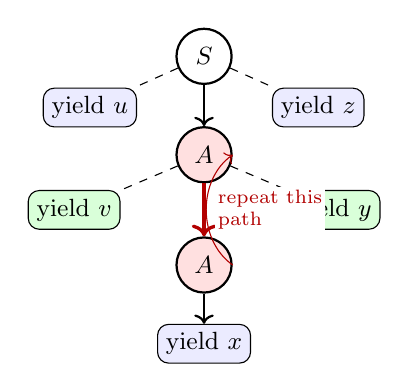
\begin{tikzpicture}[
      level distance=0.85cm,
      every node/.style={font=\small},
      state/.style={circle,draw,thick,minimum size=0.7cm},
      piece/.style={rounded corners,draw,fill=blue!8,inner sep=3pt}]
      \node[state] (S) at (0,2.8) {$S$};
      \node[state,fill=red!12] (Ao) at (0,1.55) {$A$};
      \node[state,fill=red!12] (Ai) at (0,0.15) {$A$};
      \node[piece] (u) at (-1.45,2.15) {yield $u$};
      \node[piece] (z) at (1.45,2.15) {yield $z$};
      \node[piece,fill=green!15] (v) at (-1.65,0.85) {yield $v$};
      \node[piece,fill=green!15] (y) at (1.65,0.85) {yield $y$};
      \node[piece] (x) at (0,-0.85) {yield $x$};
      \draw[->,thick] (S)--(Ao);
      \draw[->,very thick,red!70!black] (Ao)--(Ai);
      \draw[->,thick] (Ai)--(x);
      \draw[dashed] (S)--(u); \draw[dashed] (S)--(z);
      \draw[dashed] (Ao)--(v); \draw[dashed] (Ao)--(y);
      \draw[->,red!70!black,bend left=55]
        (Ai.east) to node[right,xshift=3pt,font=\scriptsize,align=left,
          fill=white,inner sep=1pt]
        {repeat this\\path} (Ao.east);
    \end{tikzpicture}
    \column{0.49\textwidth}
    The repeated variable creates a derivation loop:
    \[
      A\Rightarrow^*vAy.
    \]
    \pause
    \begin{align*}
      i=0:&\quad uxz,\\
      i=1:&\quad uvxyz,\\
      i=2:&\quad uvvxyyz,\\
      i=3:&\quad uvvvxyyyz.
    \end{align*}
    \begin{block}{Analogy with regular pumping}
      A repeated DFA state pumps one loop substring. A repeated CFG variable
      pumps the material produced on \emph{both sides} of the nested copy:
      $v$ and $y$.
    \end{block}
  \end{columns}
\end{frame}

\begin{frame}{Formal CFL Pumping Lemma}
  \small
  \begin{block}{Theorem}
    If $L$ is context-free, then there exists a pumping length $p\ge1$ such that every
    $s\in L$ with $|s|\ge p$ can be written
    \[
      s=uvxyz
    \]
    so that:
    \begin{enumerate}
      \item $|vxy|\le p$;
      \item $|vy|>0$; and
      \item $uv^ixy^iz\in L$ for every $i\ge0$.
    \end{enumerate}
  \end{block}
  \pause
  \begin{alertblock}{Compare with the regular pumping lemma}
    The CFL lemma pumps two pieces, $v$ and $y$, using the same exponent. The bounded window $vxy$
    may occur anywhere in $s$; it is not forced into the first $p$ symbols.
  \end{alertblock}
\end{frame}

\begin{frame}{The CFL Pumping Game}
  To prove that $L$ is not context-free, argue by contradiction:
  \begin{enumerate}
    \item \textbf{Opponent chooses} an arbitrary pumping length $p$.
    \item \textbf{You choose} a strategic $s\in L$ with $|s|\ge p$.
    \pause
    \item \textbf{Opponent chooses} any split $s=uvxyz$ satisfying
      $|vxy|\le p$ and $|vy|>0$.
    \pause
    \item \textbf{You choose}, after seeing the split, some $i\ge0$ for which
      $uv^ixy^iz\notin L$.
  \end{enumerate}
  \begin{alertblock}{Quantifier discipline}
    Your witness string must defeat \emph{every} legal decomposition. Choosing one convenient split
    and breaking it proves nothing.
  \end{alertblock}
\end{frame}

\begin{frame}{Game Comparison: Regular Versus Context-Free}
  \small
  \begin{center}
  \begin{tabular}{L{5.0cm}L{5.0cm}}
    \toprule
    Regular pumping lemma & CFL pumping lemma \\
    \midrule
    Split $s=xyz$ & Split $s=uvxyz$ \\
    Pump one substring: $xy^iz$ & Pump two substrings: $uv^ixy^iz$ \\
    $|xy|\le p$ forces $y$ near the left end & $|vxy|\le p$ gives a floating bounded window \\
    $|y|>0$ & $|vy|>0$; either $v$ or $y$ may be empty \\
    Opponent chooses the legal split & Opponent chooses the legal split \\
    You choose $i$ after seeing the split & You choose $i$ after seeing the split \\
    \bottomrule
  \end{tabular}
  \end{center}
  Both lemmas are necessary conditions, primarily useful for proving nonmembership in a language class.
\end{frame}

\begin{frame}{Example 1: $\{a^n b^n c^n\mid n\ge0\}$ Is Not Context-Free}
  \small
  Assume the language is context-free and let $p$ be its pumping length. Choose
  \[
    s=a^p b^p c^p.
  \]
  \pause
  For any legal $s=uvxyz$, the window $vxy$ has length at most $p$, so it cannot contain both an
  $a$ and a $c$: the entire block $b^p$ lies between them. Thus $v$ and $y$ affect symbols from at
  most two of the three blocks.

  Pump down with $i=0$. Since $|vy|>0$, at least one block loses a symbol, while at least one other
  block remains of length $p$. Deletion preserves the order $a^*b^*c^*$, but the three counts cannot
  all remain equal. Therefore
  \[
    uv^0xy^0z=uxz\notin L,
  \]
  contradicting the pumping lemma. Hence the language is not context-free.
\end{frame}

\begin{frame}{Example 2: Unary Perfect Squares Are Not Context-Free}
  Let
  \[
    L=\{a^{n^2}\mid n\ge0\}.
  \]
  Assume $L$ is context-free with pumping length $p$, and choose $s=a^{p^2}$.
  For any legal decomposition $s=uvxyz$, let
  \[
    d=|v|+|y|.
  \]
  The pumping conditions give $1\le d\le p$. Pumping up with $i=2$ produces a string of length
  \[
    p^2+d.
  \]
  But
  \[
    p^2<p^2+d\le p^2+p<(p+1)^2.
  \]
  Its length lies strictly between consecutive perfect squares, so $uv^2xy^2z\notin L$.
  Therefore $L$ is not context-free.
\end{frame}

\begin{frame}{Example 3: A Coupled Three-Block Language}
  \small
  Let
  \[
    L=\{a^n b^n c^{2n}:n\ge0\}.
  \]
  Assume $L$ is context-free with pumping length $p$, and choose
  $s=a^p b^p c^{2p}$. Any window $vxy$ of length at most $p$ touches at most
  two adjacent blocks, so it cannot alter all three counts.

  Pump down with $i=0$. At least one symbol is deleted because $|vy|>0$.
  \begin{itemize}
    \item If an $a$ or $b$ is deleted without equal changes to both, then
      $|a|=|b|$ fails.
    \item If the $a$- and $b$-counts both decrease equally, the untouched
      $c$-count is no longer twice the new $a$-count.
    \item If only the $b$/$c$ region is affected, either $|a|=|b|$ fails or,
      when no $b$ is deleted, $|c|=2|a|$ fails.
  \end{itemize}
  Thus every legal split can be defeated, so $L$ is not context-free.
\end{frame}

\begin{frame}{Example 4: Quadratically Related Blocks}
  \small
  Let
  \[
    L=\{a^n b^{n^2}:n\ge0\}.
  \]
  Assume $L$ is context-free with pumping length $p$. Set $N=p+1$ and choose
  $s=a^N b^{N^2}$. For an arbitrary legal split, let
  \[
    \alpha=|vy|_a,\qquad \beta=|vy|_b.
  \]
  Then $1\le\alpha+\beta\le p$. Pump down. If the resulting string remained
  in $L$, its counts would have to satisfy
  \[
    N^2-\beta=(N-\alpha)^2,
    \quad\text{so}\quad
    \beta=2N\alpha-\alpha^2.
  \]
  If $\alpha=0$, the equation requires $\beta=0$, contradicting
  $|vy|>0$. If $\alpha\ge1$, then $\alpha\le p=N-1$ and
  \[
    2N\alpha-\alpha^2=\alpha(2N-\alpha)\ge2N-1>p\ge\beta,
  \]
  again impossible. Hence $L$ is not context-free.
\end{frame}

\begin{frame}{Example 5: The Copy Language $\{ww\}$}
  \small
  Let $L=\{ww:w\in\{a,b\}^*\}$. Assume $L$ is context-free with pumping
  length $p$, and choose
  \[
    s=a^pb^pa^pb^p=(a^pb^p)(a^pb^p).
  \]
  A window $vxy$ of length at most $p$ lies in one block or crosses one
  boundary; it cannot reach two corresponding blocks.
  \begin{itemize}
    \item Pump down. If all four runs remain nonempty, at most two adjacent
      run lengths change. But any square in $a^+b^+a^+b^+$ must have its first
      and third run lengths equal and its second and fourth run lengths equal.
      At least one equality is destroyed.
    \item If pumping down would delete an entire length-$p$ run, then
      $|vy|=p$, $x=\varepsilon$, and the pumpable material is exactly that
      run. Pump up instead; precisely one run doubles, again destroying the
      required pair of equal run lengths.
  \end{itemize}
  Thus every legal decomposition has a bad pumping exponent, so $L$ is not
  context-free.
\end{frame}

\begin{frame}{Example 6: Two Crossed Dependencies}
  \small
  Let
  \[
    L=\{a^n b^m c^n d^m:n,m\ge1\}.
  \]
  Membership requires the distant pairs $|a|=|c|$ and $|b|=|d|$. Assume
  $L$ is context-free with pumping length $p$, and choose
  \[
    s=a^pb^pc^pd^p.
  \]
  Since $|vxy|\le p$, the pumpable window touches at most two adjacent blocks.
  It therefore cannot touch both $a$ and $c$, nor both $b$ and $d$.
  Pump down with $i=0$. Because $|vy|>0$, at least one block count decreases,
  while its distant dependent partner remains $p$. Consequently either
  $|a|\ne|c|$ or $|b|\ne|d|$, so
  \[
    uxz\notin L.
  \]
  This contradiction proves that $L$ is not context-free.
\end{frame}

\begin{frame}{Example 7: Strictly Increasing Block Counts}
  \small
  Let
  \[
    L=\{a^i b^j c^k:i<j<k\}.
  \]
  Assume $L$ is context-free with pumping length $p$, and choose the
  deliberately tight gaps
  \[
    s=a^p b^{p+1}c^{p+2}.
  \]
  For an arbitrary split, let $\Delta_a,\Delta_b,\Delta_c$ be the numbers of
  $a$'s, $b$'s, and $c$'s in $vy$. The bounded window cannot touch all three
  blocks, and $|vy|>0$, so these three changes are not all equal.
  \begin{itemize}
    \item Pumping up preserves both inequalities only if
      $\Delta_a\le\Delta_b\le\Delta_c$.
    \item Pumping down preserves both inequalities only if
      $\Delta_a\ge\Delta_b\ge\Delta_c$.
  \end{itemize}
  Both conditions can hold only when
  $\Delta_a=\Delta_b=\Delta_c$, which is impossible here. Hence either
  $i=2$ or $i=0$ violates a strict inequality, proving $L$ non-context-free.
\end{frame}

\begin{frame}{Pumping-Lemma Pitfalls and Limitations}
  \small
  \begin{itemize}
    \item Do not choose the decomposition; the proof must cover all legal $u,v,x,y,z$.
    \item Do not assume both $v$ and $y$ are nonempty; only $|vy|>0$ is guaranteed.
    \item Pump $v$ and $y$ with the same exponent $i$.
    \item The window $vxy$ may cross one or more symbol boundaries; justify every case.
    \item Choose $i$ after the opponent reveals the split. Often $i=0$ is cleaner than $i=2$.
    \item The lemma is necessary, not sufficient: satisfying it does not prove that a language is context-free.
  \end{itemize}
  \begin{block}{When the lemma is inconclusive}
    Try closure properties, intersection with a regular language, Ogden's lemma, or a direct structural argument.
  \end{block}
\end{frame}

\begin{frame}{Why Non-CFL Proofs Matter in Software Systems}
  \small
  A context-free parser has one stack-like source of unbounded memory. Some
  useful program constraints require comparisons that are not naturally
  context-free.
  \begin{center}
  \begin{tabular}{L{4.2cm}L{6.0cm}}
    \toprule
    Constraint & Typical implementation \\
    \midrule
    Proper nesting of parentheses and blocks & CFG parser or pushdown
      automaton \\
    A declared identifier must be used consistently & Symbol table and
      semantic analysis \\
    Function call arguments must match a declaration & Type checking after
      parsing \\
    Two arbitrarily long regions must be exact copies & Explicit comparison,
      hashes, or a later validation pass \\
    Several distant counts must agree simultaneously & Attributes, counters,
      or general program logic \\
    \bottomrule
  \end{tabular}
  \end{center}
  \begin{block}{Engineering lesson}
    Compiler front ends deliberately separate context-free syntax from
    context-sensitive semantic checks. A non-CFL proof explains why merely
    adding more CFG productions cannot enforce every desired constraint.
  \end{block}
\end{frame}

% ==========================================
% Part 9: Applications
% ==========================================
\section{Applications and Grammar Notation}

\begin{frame}{BNF and EBNF}
  Backus--Naur Form is a notation for CFG productions:
  \begin{align*}
    \texttt{<assignment>} &\mathrel{::=} \texttt{<id> = <expression>}\\
    \texttt{<id>} &\mathrel{::=} \texttt{x | y | z}.
  \end{align*}
  \pause
  Extended BNF adds notation for repetition and optional material. For example,
  \[
    \langle\mathrm{list}\rangle ::= \langle\mathrm{id}\rangle
      \{\,\texttt{","}\ \langle\mathrm{id}\rangle\,\}
  \]
  can be expanded into ordinary CFG productions:
  \[
    L\to \mathrm{id}\,R,
    \qquad
    R\to ,\,\mathrm{id}\,R\mid\varepsilon.
  \]
  EBNF conventions vary between standards, so braces, brackets, and parentheses must be defined.
\end{frame}

\begin{frame}{CFGs in a Compiler Pipeline}
  \begin{center}
  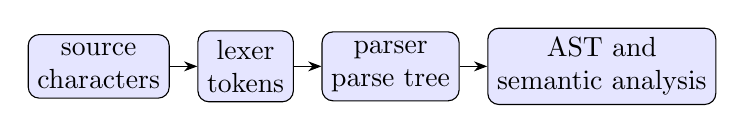
\begin{tikzpicture}[node distance=0.35cm and 0.35cm,
    box/.style={draw,rounded corners,fill=blue!10,minimum height=0.8cm,align=center},
    >=Stealth]
    \node[box] (src) {source\\characters};
    \node[box,right=of src] (lex) {lexer\\tokens};
    \node[box,right=of lex] (parse) {parser\\parse tree};
    \node[box,right=of parse] (ast) {AST and\\semantic analysis};
    \draw[->] (src)--(lex); \draw[->] (lex)--(parse); \draw[->] (parse)--(ast);
  \end{tikzpicture}
  \end{center}
  \pause
  \begin{itemize}
    \item Lexical rules are usually regular and identify tokens such as identifiers and numbers.
    \item A CFG organizes tokens into nested syntactic structure.
    \item Semantic analysis checks properties not conveniently captured by a CFG, such as types,
      declarations, and scope.
  \end{itemize}
  \begin{alertblock}{Syntax is not semantics}
    A program can be grammatically valid but still contain an undeclared variable or type error.
  \end{alertblock}
\end{frame}

\begin{frame}{Top-Down and Bottom-Up Views}
  A derivation begins with $S$ and expands variables until the input string appears. This is a
  \textbf{top-down} view of syntax.
  \begin{itemize}
    \item A top-down parser predicts which production should expand the current variable.
    \item A bottom-up parser starts from the input and repeatedly recognizes substrings corresponding
      to production right-hand sides, eventually reducing to $S$.
  \end{itemize}
  \begin{block}{Connection to the next unit}
    Pushdown automata provide the machine model for context-free languages. Their stack records
    unfinished grammatical structure during recognition or parsing.
  \end{block}
\end{frame}

% ==========================================
% Review
% ==========================================
\section{Review and Exercises}

\begin{frame}{Concept Checks}
  \small
  \begin{enumerate}
    \item Is $S$ always a sentential form? Is it always a sentence?
    \item Why do two arbitrary derivations of the same string not necessarily prove ambiguity?
    \item Which labels may occur at the leaves of a partial derivation tree but
      not a completed derivation tree?
    \item Does an ambiguous grammar necessarily generate an inherently ambiguous language?
    \item Does conversion to CNF or GNF guarantee an unambiguous grammar?
    \item How does Viterbi CKY differ from Boolean membership CYK?
    \item Which part of the expression grammar enforces multiplication precedence?
    \item Why can a CFG describe syntax but not all static semantic rules of a programming language?
  \end{enumerate}
\end{frame}

\begin{frame}{Construction Exercises}
  \small
  \begin{enumerate}
    \item Give a leftmost derivation of $000111$ using $S\to0S1\mid\varepsilon$.
    \item Draw a partial derivation tree with frontier $0S0$, then complete it
      to a tree for $0110$ using
      $S\to0S0\mid1S1\mid0\mid1\mid\varepsilon$.
    \item Design a CFG for $\{0^i1^j\mid i,j\ge0\}$ and explain why it is correct.
    \item For $S\to SS\mid a$, give two leftmost derivations of $aaa$.
    \item Modify the unambiguous expression grammar so exponentiation $\mathbin{\uparrow}$ has higher
      precedence than multiplication and is right-associative.
    \item Prove, using two inclusions, that $S\to aSb\mid\varepsilon$ generates
      $\{a^n b^n\mid n\ge0\}$.
  \end{enumerate}
\end{frame}

\begin{frame}{Exercises: Simplifying CFGs}
  \small
  \begin{enumerate}
    \item In
      \[
        S\to ABC\mid d,\quad A\to a\mid\varepsilon,\quad
        B\to bB\mid\varepsilon,\quad C\to c,
      \]
      find all nullable variables and list the rules obtained from
      $S\to ABC$ when null productions are removed.
    \item Eliminate unit productions from
      \[
        S\to A\mid d,\qquad A\to B\mid a,\qquad B\to bB\mid c.
      \]
    \item Identify the useless variables in
      \[
        S\to AB\mid a,\quad A\to a,\quad B\to b,\quad
        C\to cC\mid c,\quad D\to dD.
      \]
    \item Explain why the generating-symbol pass is normally performed before
      the reachability pass.
  \end{enumerate}
\end{frame}

\begin{frame}{Exercises: CNF, GNF, and $s$-Grammars}
  \small
  \begin{enumerate}
    \item Which of the rules below are permitted in CNF? Explain each answer.
      \[
        A\to BC,\quad A\to a,\quad A\to aB,\quad A\to B,
        \quad A\to BCD.
      \]
    \item Convert $S\to aSb\mid\varepsilon$ to CNF, using the standard fresh
      start-symbol convention to preserve $\varepsilon$.
    \item Convert the grammar
      \[
        S\to AB\mid b,\qquad A\to aA\mid a,\qquad B\to bB\mid b
      \]
      to GNF by substituting the productions for $A$ into $S\to AB$.
    \item Explain why $S\to aA\mid aB$, $A\to b$, $B\to c$ is in GNF but is
      not an $s$-grammar.
    \item Prove that a GNF leftmost derivation of a terminal word of length
      $n$ uses exactly $n$ production steps.
    \item Run CYK on $abab$ using
      $S\to AX\mid AB$, $X\to SB$, $A\to a$, and $B\to b$.
      Does the grammar generate the string?
  \end{enumerate}
\end{frame}

\begin{frame}{Exercises: CFL Properties}
  \small
  \begin{enumerate}
    \item For a CFL $L$ and regular language $R$, which are guaranteed to be context-free:
      $L\cup R$, $L\cap R$, $L\setminus R$, and $R\setminus L$?
    \item Let $L_1=L(G_1)$ and $L_2=L(G_2)$. Give grammar constructions for
      $L_1\cup L_2$, $L_1L_2$, and $L_1^*$.
    \item Construct a CFG for
      $\{a^i b^j c^k\mid i=j\text{ or }j=k\}$ using union closure.
    \item Explain why closure under complement, together with union closure, would imply closure under intersection.
    \item Classify each CFG question as decidable or undecidable: membership, emptiness, finiteness,
      universality, equivalence, and ambiguity.
    \item Why does nonclosure under intersection not mean that the intersection of every two CFLs is non-context-free?
  \end{enumerate}
\end{frame}

\begin{frame}{Exercises: CFL Pumping Lemma}
  \small
  \begin{enumerate}
    \item Use the CFL pumping lemma to prove
      $\{0^n1^n0^n\mid n\ge0\}$ is not context-free.
    \item Prove that $\{a^{n^3}\mid n\ge0\}$ is not context-free.
    \item A student chooses $s=a^p b^p c^p$ and writes ``let $v=a$ and $y=b$.''
      Explain the quantifier error.
    \item In a valid split $s=uvxyz$, may $v$ be empty? May $y$ be empty? May both be empty?
    \item Why does finding one decomposition that pumps successfully not prove that a language is context-free?
    \item For $s=a^p b^p c^p$, explain precisely why a window of length at most $p$ cannot touch all three blocks.
  \end{enumerate}
\end{frame}

\begin{frame}{Common Mistakes to Avoid}
  \begin{itemize}
    \item Giving examples instead of proving both language inclusions.
    \item Leaving a variable as a parse-tree leaf in a completed parse.
    \item Confusing $\varepsilon$ with the empty language $\varnothing$.
    \item Claiming ambiguity from two derivations that differ only in expansion order.
    \item Forgetting base productions, causing every derivation to continue forever.
    \item Adding precedence rules without checking associativity.
    \item Calling a grammar CNF before eliminating unit, mixed-terminal, or
      length-greater-than-two productions.
    \item Confusing GNF with an $s$-grammar; GNF alone does not require a
      unique rule for each leading terminal.
    \item Assuming that removing ambiguity from one grammar proves the language is never inherently ambiguous.
  \end{itemize}
\end{frame}

\begin{frame}{Summary}
  \begin{itemize}
    \item CFGs use recursive productions $A\to\alpha$ to generate context-free languages.
    \item Derivations describe substitution sequences; parse trees capture hierarchical structure.
    \item Grammar correctness is normally proved with soundness and completeness inclusions.
    \item Ambiguity is structural: one string has two parse trees or two leftmost derivations.
    \item CNF gives binary productions for proofs and CYK parsing; for a fixed
      grammar, CYK uses $O(n^3)$ time and $O(n^2)$ table space.
    \item GNF makes each production begin with a terminal, while an
      $s$-grammar adds a uniqueness condition on the leading terminal.
    \item CFLs are closed under union, concatenation, star, and intersection with regular languages,
      but not under arbitrary intersection or complement.
    \item The CFL pumping lemma pumps two bounded pieces and is used to prove languages non-context-free.
    \item Carefully designed variables encode precedence, associativity, nesting, and statement structure.
    \item CFG membership is decidable, while equivalence, universality, and ambiguity are undecidable.
  \end{itemize}
\end{frame}

\appendix
\section{Appendix: Solutions and Optional Material}

\begin{frame}{Appendix Road Map}
  \begin{itemize}
    \item Deeper motivation: language classes, compiler phases, and the
      limits of automatic program analysis;
    \item Short answers and solution blueprints for the exercises;
    \item advanced theorems about deterministic CFLs, semilinearity,
      strengthened pumping, and structural representations;
    \item surprising examples that separate closely related language classes;
    \item fully worked, newly phrased book-style challenge problems;
    \item advanced or enrichment slides that may be omitted in a shorter
      classroom delivery;
    \item guidance for selecting a compact subset of examples and
      supplementary references.
  \end{itemize}
  \begin{block}{Presentation use}
    Stop at the preceding Summary slide for the core lecture. Continue into
    this appendix only when time permits or when reviewing exercises.
  \end{block}
\end{frame}

\subsection{Deeper Motivation: Languages, Compilers, and Computation}

\begin{frame}{The Chomsky Hierarchy: What Memory Makes Possible}
  \small
  Language classes classify \emph{sets of strings}, not entire application
  areas. More powerful models can enforce more kinds of constraints.
  \begin{center}
  \begin{tabular}{L{2.6cm}L{3.0cm}L{4.3cm}}
    \toprule
    Language class & Equivalent recognizer & Memory available \\
    \midrule
    Type 3: regular & Finite automaton & Finitely many states; no auxiliary stack \\
    Type 2: context-free & Nondeterministic PDA & Finite control and one unbounded stack \\
    Type 1: context-sensitive & Nondeterministic linear bounded automaton (LBA)
      & Read/write workspace bounded by $O(n)$ cells for input length $n$ \\
    Type 0: recursively enumerable & Turing machine & Unbounded read/write tape;
      each finite computation uses only finitely many cells \\
    \bottomrule
  \end{tabular}
  \end{center}
  \pause
  \[
    \mathrm{REG}\subsetneq\mathrm{CFL}\subsetneq\mathrm{CSL}
      \subsetneq\mathrm{Decidable}\subsetneq\mathrm{Recognizable}.
  \]
  Recursively enumerable means \emph{Turing-recognizable}, not necessarily
  decidable. The decidable class is a useful extra distinction, not a fifth
  numbered grammar type.
  \par\smallskip
  {\scriptsize Empty-word convention: allow the isolated start rule
  $S_0\to\varepsilon$ when needed so the displayed inclusions include
  languages containing $\varepsilon$. See
  \paperlink{https://www.cs.utexas.edu/~cline/ear/automata/CS341-Fall-2004-Packet/1-LectureNotes.pdf}
  {UT Austin notes: language hierarchy and automata}.}
\end{frame}

\begin{frame}{A Compiler Uses Several Kinds of Reasoning}
  \small
  Compilation translates source into a target representation while
  preserving the required behavior. The target may be assembly, machine
  code, bytecode, or another source language.
  \begin{center}
  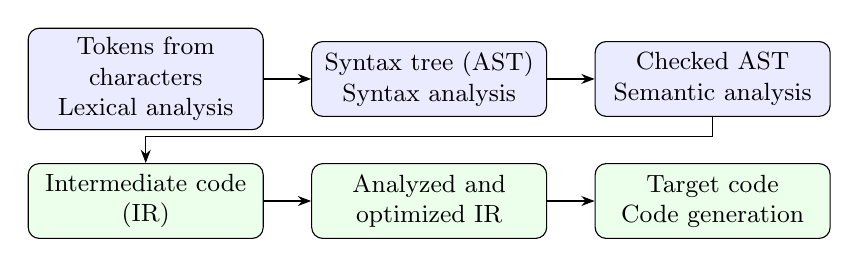
\begin{tikzpicture}[>=Stealth,
      box/.style={draw,rounded corners,fill=blue!8,align=center,
        text width=2.75cm,minimum height=0.95cm,font=\small}]
    \node[box] (lex) at (0,0) {Tokens from characters\\Lexical analysis};
    \node[box] (parse) at (3.6,0) {Syntax tree (AST)\\Syntax analysis};
    \node[box] (sem) at (7.2,0) {Checked AST\\Semantic analysis};
    \node[box,fill=green!8] (ir) at (0,-1.55) {Intermediate code\\(IR)};
    \node[box,fill=green!8] (opt) at (3.6,-1.55) {Analyzed and\\optimized IR};
    \node[box,fill=green!8] (target) at (7.2,-1.55) {Target code\\Code generation};
    \draw[->] (lex)--(parse); \draw[->] (parse)--(sem);
    \draw[->] (sem.south) -- ++(0,-0.25) -| (ir.north);
    \draw[->] (ir)--(opt); \draw[->] (opt)--(target);
  \end{tikzpicture}
  \end{center}
  \pause
  The front end analyzes source; later stages transform and emit code.
  Passes may interleave, with optimization at several representations.
  Execution is separate, though JIT compilation occurs during execution.
  \begin{alertblock}{Not one Chomsky type per compiler phase}
    Regular token rules and CFG syntax are useful design choices.
    Semantic checking and optimization are algorithms over program data,
    not automatically Type 1 and Type 0 language recognizers.
  \end{alertblock}
  {\scriptsize Source: \paperlink{https://www.cs.cornell.edu/courses/cs4120/2023sp/notes/intro/}
  {Cornell CS 4120: anatomy of a compiler}.}
\end{frame}

\begin{frame}{Lexing: Finite Memory, Not No Memory}
  \small
  In a small C-like language, the character sequence
  \[
    \texttt{int count = 123;}
    \quad\longmapsto\quad
    \mathrm{INT},\ \mathrm{ID}(\texttt{count}),\ \mathrm{ASSIGN},\
      \mathrm{NUM}(123),\ \mathrm{SEMI}.
  \]
  For example, digit strings use $DD^*$, where $D=\{0,\ldots,9\}$;
  identifiers may use $A(A\cup D)^*$, where $A$ is a chosen letter set.
  A finite automaton remembers \emph{which pattern prefix has been seen}.
  \pause
  \begin{block}{Token boundaries and priorities matter}
    Under longest-match rules, \texttt{integer} is one identifier, not
    keyword \texttt{int} followed by \texttt{eger}. A keyword rule can win
    an equal-length tie for \texttt{int}. Lexeme storage and source positions
    are implementation bookkeeping beyond finite-state recognition.
  \end{block}
  \pause
  \textbf{Beyond compilers:} fixed-format IDs, literal/regular-expression
  searches, and fixed byte signatures in network traffic are useful regular
  pattern tasks. A format match alone does not establish that an email is
  deliverable, a URL is reachable, or a packet is safe.
  \par\smallskip
  \textbf{Tool connection:} Lex/Flex-style scanners turn token patterns into
  scanning code. Not all language-specific lexing features are purely regular.
  \par\smallskip
  {\scriptsize Source: \paperlink{https://westes.github.io/flex/manual/Matching.html}
  {Flex manual: longest match and rule priority}.}
\end{frame}

\begin{frame}{Parsing: A Stack for Unbounded Nesting}
  \small
  Token recognition cannot by itself check arbitrary nesting. A stack can
  remember pending delimiters and require the right kind of closer:
  \[
    [\{\}]\quad\text{is properly nested},\qquad
    [\{]\}\quad\text{is not}.
  \]
  A CFG describes structure; the resulting parse tree or AST determines
  grouping, for example before arithmetic evaluation.
  \pause
  \begin{block}{Applications and their boundaries}
    \begin{itemize}
      \item \textbf{JSON:} objects and arrays nest recursively; grammar-based
        parsing checks syntax, not an application's schema or business rules.
      \item \textbf{XML:} nesting is only part of well-formedness; matching
        arbitrary start/end tag names is an additional explicit constraint.
      \item \textbf{HTML:} browser parsing includes specified error recovery
        and tree-building rules, not just checking balanced tags.
      \item \textbf{Natural language:} CFG phrase structure is a useful model
        of clauses, not a complete theory of meaning or translation.
    \end{itemize}
  \end{block}
  \pause
  \textbf{Tools:} Yacc/Bison generate parsers; grammar conflicts still matter.
  \par\smallskip
  {\scriptsize Sources: \paperlink{https://www.gnu.org/software/bison/manual/html_node/Language-and-Grammar.html}{Bison};
  \paperlink{https://www.rfc-editor.org/rfc/rfc8259}{JSON (RFC 8259)};
  \paperlink{https://www.w3.org/TR/xml/}{XML};
  \paperlink{https://html.spec.whatwg.org/multipage/parsing.html}{HTML parsing}.}
\end{frame}

\begin{frame}{Semantic Checks: Structure Is Not Enough}
  \small
  Suppose a toy language uses the declaration rule
  $\mathrm{Decl}\to\mathrm{Type}\ \mathrm{ID}\ \texttt{=}\
      \mathrm{Expr}\ \texttt{;}$.
  \par\smallskip
  It allows integer and string literals as expressions but forbids assigning
  a string to an integer variable. Then \texttt{int x = "hello";}
  fits the syntax while violating its type rules.
  \pause
  \begin{block}{What the semantic pass adds}
    Symbol tables record declarations and scopes; typing rules check
    expressions against expected types. Checks reject undeclared names,
    incompatible assignments, or forbidden duplicate declarations.
    Shadowing and overloading policies vary by language.
  \end{block}
  \pause
  \begin{alertblock}{Two meanings of ``context-sensitive''}
    Dependence on declarations is not a proof of Type 1 membership: that
    needs an encoding and a linear-space recognizer. Compilers use semantic
    rules and data structures, not normally a context-sensitive grammar parser.
  \end{alertblock}
  Static checks do not guarantee termination or intended behavior.
  A game's ``key present and switch on'' test is likewise a state predicate,
  not automatically a Type 1 language.
  \par\smallskip
  {\scriptsize Reading: \paperlink{https://www.cs.cornell.edu/courses/cs4120/2026sp/notes/}
  {Cornell CS 4120: semantic analysis and typing environments}.}
\end{frame}

\begin{frame}{Beyond a Stack: Reusing Input-Sized Workspace}
  \small
  A concrete Type 1 example is
  \[
    L=\{a^k b^k c^k:k\ge1\}.
  \]
  Our pumping argument shows $L$ is not context-free. Yet a machine can
  decide it using only the input cells plus finite control.
  \begin{block}{A linear-bounded marking algorithm}
    \begin{enumerate}
      \item Check that the input has the form $a^+b^+c^+$.
      \pause
      \item Mark the leftmost unmarked $a$, then one unmarked $b$, then one
        unmarked $c$. Reject if either partner is missing.
      \pause
      \item Return to the left and repeat. When no unmarked $a$ remains,
        accept iff no unmarked $b$ or $c$ remains.
    \end{enumerate}
  \end{block}
  Use marked versions $A,B,C$ of the input symbols; no extra tape region
  is needed. Each successful round removes one obligation from each block.
  \pause
  \par
  A stack accesses only its top; an LBA can revisit and mark earlier input.
  ``Bounded'' means linear in input length, not a fixed amount for all inputs.
  With finitely many configurations per input, configuration-graph
  reachability decides LBA acceptance.
  \par
  {\scriptsize This example illustrates workspace, not a required compiler
  phase. Reading: \cite{linz,hopcroft}.}
\end{frame}

\begin{frame}{General Computation: Power Comes with Limits}
  \small
  Type 0 grammars generate exactly the Turing-recognizable languages.
  A recognizer accepts members, but may run forever on nonmembers.
  Consider the language of encoded program--input pairs
  \[
    H=\{\langle P,x\rangle:P\text{ eventually halts on }x\}.
  \]
  Simulating $P(x)$ recognizes $H$: accept if the simulation halts.
  No algorithm decides $H$ correctly for every pair and always terminates.
  \pause
  \begin{exampleblock}{Why perfect reachability analysis would be impossible}
    Given $P,x$, construct a wrapper that first simulates $P(x)$, then
    executes a distinguished statement \texttt{emit(1)}.
    The statement is reachable exactly when $P(x)$ halts. An always-correct,
    always-terminating reachability checker for arbitrary programs would
    therefore decide the halting problem.
  \end{exampleblock}
  \pause
  This is a limit on \emph{all} algorithms, not merely on CFG parsers.
  Restricted cases can still be decided, and useful analyses can return
  conservative answers when they cannot establish a fact.
  \par\smallskip
  \textbf{General-purpose does not mean omnipotent.} AI and cryptography
  are application areas, not extra hierarchy levels; computational
  difficulty is not the same as undecidability.
  \par
  {\scriptsize Source: \paperlink{https://www.cs.cornell.edu/courses/cs212/2000sp/notes/lectures/l28-computability.htm}
  {Cornell: computability and limits of program analysis}.}
\end{frame}

\begin{frame}{Optimization: Safe Rewrites, Not Omniscience}
  \small
  An optimizer seeks better time, space, or energy use while preserving
  required observable behavior. Useful rewrites need not solve arbitrary logic.
  \begin{description}
    \item[Constant folding:] under exact integer arithmetic, replace
      \texttt{60 * 60 * 24} with \texttt{86400}. Machine types, overflow,
      and floating-point rules must be respected.
    \pause
    \item[Unreachable code:] remove the body of a literal \texttt{if (false)}
      branch. Removing an unused computation also requires checking
      side effects and traps.
    \pause
    \item[Loop unrolling:] a simple loop calling \texttt{work(i)} for
      $i=0,1,2$ can become \texttt{work(0); work(1); work(2);} when the
      loop variable is local and the body cannot alter control flow.
      This may reduce loop overhead but increases code size; speedup is
      not guaranteed.
  \end{description}
  \pause
  \begin{block}{Separate legality from profitability}
    Sound analyses justify \emph{whether} a rewrite preserves behavior;
    cost models and heuristics choose \emph{whether it is worthwhile}.
    Uncertainty is not permission to change the program's meaning.
  \end{block}
  \textbf{Course lesson:} choose models to fit the constraints; recognize
  limits on universal analysis. Optimization is not a Type 0 classification.
  \par\smallskip
  {\scriptsize Examples and implementation details:
  \paperlink{https://llvm.org/docs/Passes.html}{LLVM transformation passes} and
  \paperlink{https://mlir.llvm.org/docs/Canonicalization/}{MLIR canonicalization}.}
\end{frame}

\subsection{Hints and Short Answers}

\begin{frame}{Hints and Short Answers}
  \small
  \begin{enumerate}
    \item $S\Rightarrow0S1\Rightarrow00S11\Rightarrow000S111\Rightarrow000111$.
    \item The first expansion $S\Rightarrow0S0$ gives the requested partial
      tree. Complete it with the inner production $S\to1S1$, then
      $S\to\varepsilon$.
    \item $S\to AB$, $A\to0A\mid\varepsilon$, $B\to1B\mid\varepsilon$.
    \item Two leftmost derivations are
      $S\Rightarrow SS\Rightarrow SSS\Rightarrow aSS\Rightarrow aaS\Rightarrow aaa$
      and
      $S\Rightarrow SS\Rightarrow aS\Rightarrow aSS\Rightarrow aaS\Rightarrow aaa$.
    \item Keep $T\to T\times F\mid F$ and use
      $F\to A\mathbin{\uparrow}F\mid A$, $A\to(E)\mid\mathrm{id}$.
      The right recursion makes exponentiation right-associative.
    \item Use the invariant $a^kSb^k$ for soundness and apply the recursive rule exactly $n$ times
      for completeness.
  \end{enumerate}
\end{frame}

\begin{frame}{Hints: Simplifying CFGs}
  \small
  \begin{enumerate}
    \item $A$ and $B$ are nullable; $C$ and $S$ are not. Replace
      $S\to ABC$ by
      \[
        S\to ABC\mid BC\mid AC\mid C.
      \]
    \item The unit closures allow $S$ to inherit the non-unit rules of both
      $A$ and $B$, and $A$ to inherit those of $B$:
      \[
        S\to d\mid a\mid bB\mid c,\quad
        A\to a\mid bB\mid c,\quad B\to bB\mid c.
      \]
    \item $D$ is non-generating. After it is removed, $C$ is generating but
      unreachable from $S$. Thus both $C$ and $D$ are useless.
    \item Removing non-generating symbols first can remove productions and
      expose additional reachability facts. The second pass then explores only
      productions capable of participating in terminal derivations.
  \end{enumerate}
\end{frame}

\begin{frame}{Hints: CNF, GNF, and $s$-Grammars}
  \small
  \begin{enumerate}
    \item Only $A\to BC$ and $A\to a$ have CNF form.
    \item Add $S_0\to S$, then eliminate the nullable rule to obtain
      $S_0\to S\mid\varepsilon$ and $S\to aSb\mid ab$. Introduce
      $A\to a$, $B\to b$, and $X\to SB$. After eliminating $S_0\to S$, use
      \[
        S_0\to AX\mid AB\mid\varepsilon,\qquad
        S\to AX\mid AB,\quad X\to SB,\quad A\to a,\quad B\to b.
      \]
    \item Substitute $A\to aA\mid a$ into $S\to AB$ to obtain
      \[
        S\to aAB\mid aB\mid b,\quad
        A\to aA\mid a,\quad B\to bB\mid b.
      \]
      Every rule now begins with a terminal and is followed only by variables.
    \item The two $S$-productions share the same leading terminal $a$; the
      pair $(S,a)$ therefore does not select a unique production.
    \item Each GNF production introduces exactly one terminal at the left edge
      of the remaining sentential form. Starting with zero terminals and ending
      with $n$ therefore requires exactly $n$ steps.
    \item The length-one cells are
      $\{A\},\{B\},\{A\},\{B\}$. The two occurrences of $ab$ produce
      $\{S\}$, but neither length-three cell nor the length-four top cell gains
      a variable. Therefore CYK rejects $abab$.
  \end{enumerate}
\end{frame}

\begin{frame}{Hints: CFL Properties}
  \small
  \begin{enumerate}
    \item $L\cup R$, $L\cap R$, and $L\setminus R$ are guaranteed CFLs;
      $R\setminus L$ is not guaranteed context-free.
    \item Use fresh $S$ with $S\to S_1\mid S_2$, $S\to S_1S_2$, or
      $S\to S_1S\mid\varepsilon$, respectively.
    \item Take the union of a grammar for $a^n b^n c^*$ and one for $a^*b^n c^n$.
    \item If complement closure held, then
      $L_1\cap L_2=\overline{\overline{L_1}\cup\overline{L_2}}$ would be a CFL.
    \item Membership, emptiness, and finiteness are decidable; universality, equivalence, and ambiguity are undecidable.
    \item Nonclosure means that at least one counterexample pair exists, not that every pair fails.
  \end{enumerate}
\end{frame}

\begin{frame}{Hints: CFL Pumping Exercises}
  \small
  \begin{enumerate}
    \item Choose $s=0^p1^p0^p$. The bounded window cannot touch both outer
      $0$-blocks. Pumping down alters at most two adjacent blocks, so the three
      required block lengths cannot remain equal.
    \item Choose $s=a^{p^3}$. If $d=|v|+|y|$, then $1\le d\le p$, while
      $(p+1)^3-p^3=3p^2+3p+1>p$; pumping up lands between consecutive cubes.
    \item The opponent, not the student, chooses $v$ and $y$. Every legal decomposition must be handled.
    \item Either $v$ or $y$ may be empty, but $|vy|>0$ forbids both from being empty.
    \item The lemma promises the existence of some pumpable decomposition for every sufficiently long
      string; one successful split does not establish that universal condition.
    \item Touching an $a$ and a $c$ would also include all $p$ intervening $b$'s, giving length at least $p+2$.
  \end{enumerate}
\end{frame}

% ==========================================
% Appendix enrichment: advanced CFL results
% ==========================================
\subsection{Advanced Theorems and Observations}

\begin{frame}{Deterministic CFLs Behave Differently}
  \small
  A \textbf{deterministic context-free language} (DCFL) is accepted by a
  deterministic pushdown automaton. Determinism changes several familiar
  properties.
  \pause
  \begin{center}
  \begin{tabular}{L{4.0cm}L{2.5cm}L{2.5cm}}
    \toprule
    Property & CFL & DCFL \\
    \midrule
    complement & not closed & closed \\
    union and intersection & union only & not closed \\
    intersection with regular languages & closed & closed \\
    has an unambiguous grammar & not always & always \\
    \bottomrule
  \end{tabular}
  \end{center}
  \pause
  Thus
  \[
    \text{DCFL}\subsetneq\text{unambiguous CFL}
      \subsetneq\text{CFL}.
  \]
  An inherently ambiguous CFL therefore cannot be deterministic.
  \begin{alertblock}{Technical caution}
    Complementing a DPDA requires a normalized machine that consumes the
    entire input and does not diverge forever on $\varepsilon$-moves; merely
    swapping final states is not sufficient for an arbitrary presentation.
  \end{alertblock}
\end{frame}

\begin{frame}{Ogden's Lemma: Mark the Important Positions}
  \footnotesize
  The ordinary CFL pumping lemma lets the opponent hide the pumped pieces in
  an unhelpful region. Ogden's lemma strengthens it by letting us mark the
  positions that matter.
  \pause
  \begin{block}{Ogden's Lemma}
    For every CFL $L$, some $p\ge1$ has the following property. If
    $z\in L$ has at least $p$ marked positions, then
    $z=uvwxy$ so that
    \begin{enumerate}
      \item $v$ and $x$ together contain at least one marked position;
      \item $vwx$ contains at most $p$ marked positions; and
      \item $uv^iwx^iy\in L$ for every $i\ge0$.
    \end{enumerate}
  \end{block}
  \pause
  Marking every position recovers the usual pumping lemma. Strategic marking
  can force at least one pumped part into a selected block, making some
  non-CFL and inherent-ambiguity proofs possible when ordinary pumping is too
  weak.

  \paperlink{https://doi.org/10.1007/BF01694004}{Original paper: W. Ogden,
  ``A Helpful Result for Proving Inherent Ambiguity'' (1968).}
\end{frame}

\begin{frame}{Parikh's Theorem: Counts Forget Order}
  \small
  For $\Sigma=\{a_1,\ldots,a_k\}$, the \textbf{Parikh image} of a word is
  \[
    \Psi(w)=(|w|_{a_1},\ldots,|w|_{a_k}).
  \]
  It records symbol counts but discards their order.
  \pause
  \begin{block}{Parikh's Theorem}
    The Parikh image of every context-free language is a semilinear set: a
    finite union of sets of the form
    \[
      \mathbf b+n_1\mathbf p_1+\cdots+n_r\mathbf p_r,qquad n_i\ge0.
    \]
    Equivalently, every CFL has the same Parikh image as some regular
    language.
  \end{block}
  \pause
  Therefore a language whose count vectors are not semilinear cannot be
  context-free. The converse is false: semilinear counts do not capture word
  order.

  \paperlink{https://doi.org/10.1145/321356.321364}{Original paper: R. Parikh,
  ``On Context-Free Languages'' (1966).}
\end{frame}

\begin{frame}{Chomsky--Sch\"utzenberger Representation}
  \small
  Let $D_k$ be the Dyck language of correctly nested strings using $k$ types
  of parentheses.
  \pause
  \begin{block}{Representation Theorem}
    A language $L$ is context-free if and only if there exist some $k$, a
    regular language $R$, and a homomorphism $h$ such that
    \[
      L=h(D_k\cap R).
    \]
  \end{block}
  \pause
  This decomposes every CFL into three ingredients:
  \begin{enumerate}
    \item a Dyck language supplies unbounded nested memory;
    \item a regular filter $R$ restricts the permitted structural patterns;
    \item a homomorphism translates the surviving brackets into terminals.
  \end{enumerate}
  \begin{exampleblock}{Conceptual significance}
    Balanced nesting is the universal context-free mechanism; finite-state
    control and symbol translation customize it into a particular CFL.
  \end{exampleblock}

  \paperlink{https://doi.org/10.1016/S0049-237X(09)70104-1}{Chomsky and
  Sch\"utzenberger's foundational treatment.}
\end{frame}

\begin{frame}{Substitution: A Powerful Closure Principle}
  \small
  A \textbf{substitution} assigns each terminal $a\in\Sigma$ a language
  $\sigma(a)$ and extends to words by concatenation and to languages by union.
  \pause
  \begin{block}{Closure under context-free substitution}
    If $L$ is context-free and every $\sigma(a)$ is context-free, then
    $\sigma(L)$ is context-free.
  \end{block}
  \textbf{Grammar construction.} Rename all variables to be disjoint. In a
  grammar for $L$, replace each terminal $a$ by the start variable $S_a$ of a
  grammar for $\sigma(a)$, and include all those productions.
  \pause
  \begin{exampleblock}{Example}
    Let $L=\{0^n1^n:n\ge0\}$,
    $\sigma(0)=\{a^ib^i:i\ge1\}$, and
    $\sigma(1)=\{c,d\}$. Then $\sigma(L)$ consists of $n$ matched
    $a^ib^i$ blocks followed by exactly $n$ symbols chosen from $\{c,d\}$,
    and is context-free by the theorem.
  \end{exampleblock}
  Homomorphism closure is the special case in which every $\sigma(a)$ is a
  singleton language.
\end{frame}

\begin{frame}{A Surprising Decidability Boundary}
  \small
  For arbitrary CFGs, language equivalence is undecidable. Restricting the
  machines to deterministic pushdown automata changes the answer.
  \pause
  \begin{block}{S\'enizergues' Theorem}
    Equivalence of deterministic pushdown automata is decidable: there is an
    algorithm that determines whether two DPDAs accept the same language.
  \end{block}
  \pause
  The result is much deeper than DFA equivalence. It does not imply a simple
  product-and-reachability test, and it does not extend to arbitrary
  nondeterministic PDAs.
  \begin{alertblock}{Lesson}
    Two models can recognize closely related classes yet have dramatically
    different meta-problems. Determinism affects not only parsing speed but
    also what questions about machines are decidable.
  \end{alertblock}

  \paperlink{https://doi.org/10.1007/3-540-63165-8_221}{G. S\'enizergues,
  ``The Equivalence Problem for Deterministic Pushdown Automata Is
  Decidable'' (1997).}
\end{frame}

\begin{frame}{CNF Gives Quantitative Parse-Tree Bounds}
  \small
  Suppose an $\varepsilon$-free grammar is in CNF and a derivation produces a
  word of length $n\ge1$.
  \pause
  \begin{block}{Exact node and step counts}
    Its parse tree has $n$ terminal leaves, $n-1$ binary variable nodes, and
    therefore exactly
    \[
      2n-1
    \]
    production applications: $n-1$ rules of the form $A\to BC$ and $n$ rules
    of the form $A\to a$.
  \end{block}
  \pause
  If a CNF grammar with $k$ variables generates any nonempty word, then it
  generates one of length at most $2^{k-1}$. Choose a shortest word: no
  root-to-leaf path in its parse tree can repeat a variable, or the repeated
  portion could be removed to obtain a shorter word. Thus the variable height
  is at most $k$, and a binary tree of that height has at most $2^{k-1}$
  leaves.
\end{frame}

\begin{frame}{Beyond One Word: The Interchange Lemma}
  \small
  Pumping lemmas analyze repeatable structure inside one sufficiently long
  word. The \textbf{interchange lemma} instead considers a large collection
  of equal-length words in a CFL.
  \pause
  \begin{block}{Informal form}
    Within a sufficiently large collection, many words can be decomposed with
    corresponding middle regions of the same length so that exchanging those
    regions between selected words still produces words in the language.
  \end{block}
  \pause
  It is useful when every individual word appears pumpable but the language
  cannot support the many cross-combinations forced by context-free parse-tree
  structure. Like pumping and Ogden's lemma, it is a necessary condition, not
  a complete characterization of CFLs.
  \begin{exampleblock}{When to investigate it}
    The method is especially relevant for dense families involving copying,
    repetition, or many correlated choices where a single-word argument does
    not expose the contradiction.
  \end{exampleblock}

  \paperlink{https://doi.org/10.1137/0214031}{Ogden, Ross, and Winklmann,
  ``An Interchange Lemma for Context-Free Languages'' (1985).}
\end{frame}

% ==========================================
% Appendix enrichment: surprising examples
% ==========================================
\subsection{Surprising Separations and Examples}

\begin{frame}{One Marker Can Change Deterministic Parsability}
  \small
  Compare the palindrome languages
  \[
    P=\{ww^R:w\in\{0,1\}^*\},
    \qquad
    P_\#=\{w\#w^R:w\in\{0,1\}^*\}.
  \]
  Both are context-free.
  \pause
  \begin{itemize}
    \item $P_\#$ is deterministic context-free: push symbols before the
      marker, then pop and compare after the marker.
    \item $P$ is not deterministic context-free: without a marker, a
      one-stack deterministic machine cannot know when to switch from pushing
      to matching.
  \end{itemize}
  \pause

  The delimiter does not add unbounded information; it supplies one decisive
  structural event. This is why explicit separators and closing tokens often
  make programming-language syntax easier to parse deterministically.
\end{frame}

\begin{frame}{The Same Counts Can Hide Different Complexity}
  \small
  Consider
  \[
    L_1=(abc)^*,
    \qquad
    L_2=\{a^n b^n c^n:n\ge0\}.
  \]
  The first language is regular; the second is not context-free.
  \pause
  Nevertheless they have exactly the same Parikh image:
  \[
    \Psi(L_1)=\Psi(L_2)=\{(n,n,n):n\ge0\}.
  \]
  \pause
  \begin{alertblock}{What Parikh's theorem cannot see}
    Semilinearity is a necessary condition for context-freeness, not a
    sufficient one. The obstruction in $L_2$ is the ordered three-way
    dependency, not the set of possible symbol counts.
  \end{alertblock}
  This also explains why counting abstractions used in program analysis can
  prove some impossibility results but may lose essential sequencing
  information.
\end{frame}

\begin{frame}{Nested Dependencies Work; Crossed Ones Fail}
  \small
  Compare
  \[
    N=\{a^n b^m c^m d^n:n,m\ge0\}
  \]
  with
  \[
    X=\{a^n b^m c^n d^m:n,m\ge0\}.
  \]
  \pause
  $N$ is context-free, generated by
  \[
    S\to aSd\mid T,
    \qquad T\to bTc\mid\varepsilon.
  \]
  The $a/d$ dependency surrounds the $b/c$ dependency, matching stack order.
  \pause
  The language $X$ is not context-free: the required pairs cross. A stack
  that stores information for the $a/c$ comparison blocks access to the
  information needed later for $b/d$ in the wrong order.
  \begin{block}{Structural heuristic}
    A single stack naturally supports properly nested obligations. Independent
    crossed obligations are a warning sign that one stack is insufficient.
  \end{block}
\end{frame}

\begin{frame}{Nonclosure Does Not Mean ``Never''}
  \small
  CFLs are not closed under complement, but particular CFLs can still have
  context-free complements.
  \pause
  Let
  \[
    L=\{a^n b^n:n\ge0\}\subseteq\{a,b\}^*.
  \]
  Then
  \[
    \overline L=
    (\Sigma^*\setminus a^*b^*)
    \cup\{a^i b^j:0\le i<j\}
    \cup\{a^i b^j:0\le j<i\}.
  \]
  The first component is regular, and the two unequal-count components are
  context-free; union closure makes $\overline L$ context-free.
  \pause
  \begin{alertblock}{Logical distinction}
    ``The class is not closed under complement'' means that at least one CFL
    has a non-CFL complement. It does not mean every complemented CFL leaves
    the class.
  \end{alertblock}
\end{frame}

\begin{frame}{Another Classical Inherently Ambiguous CFL}
  \small
  Define
  \[
    \begin{aligned}
      K_1&=\{a^n b^m c^m d^n:n,m\ge1\},\\
      K_2&=\{a^n b^n c^m d^m:n,m\ge1\},\\
      K&=K_1\cup K_2.
    \end{aligned}
  \]
  \pause
  $K_1$ is context-free because its dependencies are nested; $K_2$ is the
  concatenation of two matched-block CFLs. Hence $K$ is context-free.
  Their overlap is
  \[
    K_1\cap K_2=\{a^n b^n c^n d^n:n\ge1\}.
  \]
  The language $K$ is a standard second example of an inherently ambiguous
  CFL: every grammar for it must assign multiple parses to some words.
  \pause
  \begin{alertblock}{Do not use an invalid shortcut}
    Showing that two convenient component grammars overlap proves their union
    grammar ambiguous, but does not by itself prove the language inherently
    ambiguous. The unavoidable-ambiguity result requires a deeper theorem.
  \end{alertblock}
\end{frame}

\begin{frame}{Maurer's Example and Unbounded Ambiguity}
  \footnotesize
  A structurally different inherently ambiguous language is
  \[
    \begin{aligned}
      M={}&\{a^n b^m a^r b^m:n,m,r\ge1\}\\
          &\cup\{a^n b^m a^n b^s:n,m,s\ge1\}.
    \end{aligned}
  \]
  The first component matches the two $b$-blocks; the second matches the two
  $a$-blocks. Their shared words include
  $(a^n b^m)^2$. Maurer gave a direct proof that no unambiguous CFG can
  generate $M$.
  \pause
  \begin{block}{A still stronger phenomenon}
    For the standard three-block language
    \[
      L=\{a^n b^n c^k:n,k\ge1\}
        \cup\{a^i b^n c^n:i,n\ge1\},
    \]
    Ogden showed that $L^*$ has \textbf{unbounded inherent ambiguity}: in
    every CFG for $L^*$, the number of parses cannot be bounded by any fixed
    constant over all words.
  \end{block}
  \pause
  Bijective renaming of terminals and reversal preserve inherent ambiguity,
  producing infinitely many equivalent variants. No regular language is
  inherently ambiguous because a DFA yields an unambiguous right-linear
  grammar.

  \paperlink{https://doi.org/10.1145/321510.321517}{Maurer's direct proof}
  \qquad
  \paperlink{https://doi.org/10.1007/BF01694004}{Ogden's strengthened result}
\end{frame}

% ==========================================
% Appendix enrichment: worked challenges
% ==========================================
\subsection{Solved Book-Style Challenges}

\begin{frame}{Challenge 1: Build a Union Language Carefully}
  \footnotesize
  \begin{block}{Problem}
    Construct a CFG for
    \[
      L=\{a^i b^j c^k:i=j\text{ or }j=k,\ i,j,k\ge1\}.
    \]
  \end{block}
  Split the condition into two CFLs. One grammar is
  \[
    \begin{aligned}
      S&\to X\mid Y,\\
      X&\to AC, & A&\to aAb\mid ab, & C&\to cC\mid c,\\
      Y&\to DB, & D&\to aD\mid a,  & B&\to bBc\mid bc.
    \end{aligned}
  \]
  $X$ generates $a^n b^n c^k$ and $Y$ generates $a^i b^n c^n$, so the union
  generates exactly $L$.
  \pause

  Every $a^n b^n c^n$ can be derived through both branches. This proves the
  displayed grammar ambiguous. The stronger claim that $L$ is inherently
  ambiguous requires a theorem about the language, not merely these two
  derivations.
\end{frame}

\begin{frame}{Challenge 2: Equal Counts in Any Order}
  \small
  \begin{block}{Problem}
    Show that
    \[
      E=\{w\in\{a,b,c\}^*:|w|_a=|w|_b=|w|_c\}
    \]
    is not context-free.
  \end{block}
  Assume $E$ is context-free and intersect it with the regular language
  $a^*b^*c^*$. Closure under intersection with regular languages would make
  the result context-free. But
  \[
    E\cap a^*b^*c^*=\{a^n b^n c^n:n\ge0\},
  \]
  which is not context-free. This contradiction proves that $E$ is not a CFL.
  \pause
  \begin{exampleblock}{Why this proof is efficient}
    Direct pumping must manage many symbol orders. The regular filter isolates
    the canonical ordered sublanguage where the known obstruction is visible.
  \end{exampleblock}
\end{frame}

\begin{frame}{Challenge 3: A Short Witness for Nonemptiness}
  \small
  \begin{block}{Problem}
    An $\varepsilon$-free CNF grammar has $k$ variables. Prove that if its
    language is nonempty, it contains a word of length at most $2^{k-1}$.
  \end{block}
  Choose a shortest generated word $w$ and a parse tree for it. If some
  variable $A$ occurs twice on one root-to-leaf path, the upper $A$ derives a
  context containing the lower $A$. Replacing the upper subtree by the lower
  subtree removes at least one productive side branch and yields a shorter
  terminal word, contradicting the choice of $w$.
  \pause

  Hence each path contains at most $k$ variable nodes. A binary tree with at
  most $k$ variable levels has at most $2^{k-1}$ terminal leaves. Since the
  yield length equals the number of terminal leaves,
  $|w|\le2^{k-1}$.
\end{frame}

\begin{frame}{Challenge 4: Decide Whether a CFL Is Infinite}
  \small
  \begin{block}{Problem}
    Give a graph-based finiteness test for a CFG.
  \end{block}
  First remove useless symbols and convert the grammar to CNF, treating
  $\varepsilon$ separately. Build a dependency graph with an edge $A\to B$
  whenever a rule for $A$ contains $B$.
  \pause
  \begin{block}{Criterion}
    The reduced language is infinite exactly when the dependency graph has a
    directed cycle reachable from the start variable.
  \end{block}
  In a reduced CNF grammar, every side variable on such a recursive cycle can
  derive a nonempty terminal word. Repeating the cycle therefore increases the
  yield length and produces infinitely many words. If there is no reachable
  cycle, derivation-tree height is bounded, so only finitely many parse trees
  and terminal words are possible.
\end{frame}

\begin{frame}{Challenge 5: Quotient by a Fixed Suffix}
  \small
  \begin{block}{Problem}
    If $L$ is context-free and $u$ is a fixed word, prove that
    \[
      L/\{u\}=\{x:xu\in L\}
    \]
    is context-free.
  \end{block}
  Let an NPDA $P$ recognize $L$. Construct $P_u$ that reads the supplied input
  $x$ exactly as $P$ does. After the input ends, $P_u$ enters a finite chain of
  control states that simulates $P$ on the fixed symbols of $u$ using
  $\varepsilon$-moves, while retaining the same stack.
  \pause

  The new machine accepts precisely when some computation of $P$ accepts
  $xu$. Therefore $L/\{u\}$ is context-free.
  \begin{exampleblock}{Generalization}
    CFLs are closed under left and right quotient with regular languages. The
    fixed-word construction is the simplest visible case of that theorem.
  \end{exampleblock}
\end{frame}

\begin{frame}{Challenge 6: CFL or Not? Use Structure First}
  \footnotesize
  Classify the following languages and justify each answer.
  \begin{enumerate}
    \item $L_1=\{a^n b^m c^m d^n:n,m\ge0\}$ is a CFL; use
      $S\to aSd\mid T$ and $T\to bTc\mid\varepsilon$.
    \pause
    \item $L_2=\{a^n b^m c^n d^m:n,m\ge0\}$ is not a CFL. For
      $a^p b^p c^p d^p$, the window $vwx$ touches at most two adjacent
      blocks. Pumping changes a block without its distant matching partner,
      so either $|a|=|c|$ or $|b|=|d|$ fails.
    \pause
    \item $L_3=\{wcw^R:w\in\{0,1\}^*\}$ is a DCFL; push before $c$ and pop
      while matching afterward.
    \pause
    \item $L_4=\{ww:w\in\{0,1\}^*\}$ is not a CFL; the second half must copy
      the first in the same order rather than reverse stack order.
  \end{enumerate}
  \begin{alertblock}{Exam strategy}
    Before choosing a proof tool, ask whether the dependencies are nested,
    separated by a marker, or crossed. That structural diagnosis often
    determines the correct construction or contradiction.
  \end{alertblock}
\end{frame}

\begin{frame}{About the Book-Style Challenges}
  \small
  The preceding exercises are newly phrased and solved from recurring themes
  in standard formal-language texts rather than copied verbatim:
  \begin{itemize}
    \item grammar construction by union and structural decomposition;
    \item regular filtering to expose a known non-CFL;
    \item CNF parse-tree bounds and grammar finiteness;
    \item quotient closure and PDA simulation; and
    \item nested versus crossed stack dependencies.
  \end{itemize}
  \pause
  \begin{block}{Recommended workflow}
    Try a grammar or PDA construction first when obligations are nested. Use
    closure with a regular filter when it isolates a standard hard language.
    Reserve pumping or Ogden's lemma for cases where constructive approaches
    fail and every legal decomposition can be controlled.
  \end{block}
\end{frame}

\begin{frame}{Appendix Guide: Optional Theory Slides}
  \footnotesize
  For a shorter first course, retain the formal definitions and omit or move
  the following enrichment slides to reading material:
  \begin{columns}[T]
    \column{0.48\textwidth}
    \begin{itemize}
      \item \textit{Reusable Grammar-Design Patterns II}
      \item \textit{Parse Trees and Abstract Syntax Trees}
      \item \textit{The Same Ambiguity as Leftmost Derivations}
      \item \textit{The Dangling-Else Ambiguity}
      \item \textit{Grammar Ambiguity Versus Inherent Ambiguity}
      \item \textit{Understanding an Inherently Ambiguous Language}
      \item \textit{Predictive Recognition for an $s$-Grammar}
    \end{itemize}
    \column{0.48\textwidth}
    \begin{itemize}
      \item \textit{What Fails the $s$-Grammar Test?}
      \item \textit{Meaning of Equivalent Normal Form}
      \item \textit{A Systematic GNF Conversion Outline}
      \item \textit{GNF Versus an $s$-Grammar}
      \item \textit{Other Useful Grammar Forms and Restrictions}
      \item \textit{Important CKY/CYK Extensions}
      \item \textit{CYK in Practice and Important Alternatives}
    \end{itemize}
  \end{columns}
  These slides add depth but are not prerequisites for the core CFG--PDA
  equivalence normally taught next.
\end{frame}

\begin{frame}{Appendix Guide: Optional Examples and Review}
  \footnotesize
  \begin{block}{Keep as the minimum conceptual spine}
    CFG definition; derivations; complete and partial derivation trees; one
    ambiguity example; simplification procedures; CNF; the core CYK recurrence;
    CFL closure/nonclosure; the pumping theorem and game; and one complete
    non-CFL proof.
  \end{block}
  \begin{block}{Select rather than present all}
    \begin{itemize}
      \item Keep \textit{Worked CNF Conversion} and either the worked CYK table
        or the CYK exercise, not necessarily both.
      \item Keep pumping Example~1 and choose only one of Examples~2--7 based
        on the examination level.
      \item Choose either \textit{Worked Closure Examples} or
        \textit{Filtering a CFL with a Regular Language}.
      \item Move all hint slides to an appendix or distribute them after class.
      \item Omit BNF/EBNF and compiler-pipeline slides if those topics are
        already covered in a compiler course.
    \end{itemize}
  \end{block}
\end{frame}

\begin{frame}{References: Advanced CFL Results}
  \scriptsize
  \begin{thebibliography}{9}
    \bibitem{parikh}
      Rohit J. Parikh,
      \newblock \paperlink{https://doi.org/10.1145/321356.321364}
      {\emph{On Context-Free Languages}},
      \newblock Journal of the ACM, 13(4), 1966.

    \bibitem{ogden}
      William Ogden,
      \newblock \paperlink{https://doi.org/10.1007/BF01694004}
      {\emph{A Helpful Result for Proving Inherent Ambiguity}}, 1968.

    \bibitem{maurer}
      Herman A. Maurer,
      \newblock \paperlink{https://doi.org/10.1145/321510.321517}
      {\emph{A Direct Proof of the Inherent Ambiguity of a Simple
      Context-Free Language}}, 1969.

    \bibitem{cs}
      Noam Chomsky and Marcel-Paul Sch\"utzenberger,
      \newblock \paperlink{https://doi.org/10.1016/S0049-237X(09)70104-1}
      {\emph{The Algebraic Theory of Context-Free Languages}}, 1959.

    \bibitem{interchange}
      William Ogden, Rockford J. Ross, and Karl Winklmann,
      \newblock \paperlink{https://doi.org/10.1137/0214031}
      {\emph{An Interchange Lemma for Context-Free Languages}}, 1985.

    \bibitem{senizergues}
      G\'eraud S\'enizergues,
      \newblock \paperlink{https://doi.org/10.1007/3-540-63165-8_221}
      {\emph{The Equivalence Problem for Deterministic Pushdown Automata Is
      Decidable}}, 1997.
  \end{thebibliography}
\end{frame}

\begin{frame}{References: Parsing Algorithms}
  \footnotesize
  \begin{thebibliography}{9}
    \bibitem{jurafsky-martin}
      Daniel Jurafsky and James H. Martin,
      \newblock \emph{Speech and Language Processing}, 3rd-edition draft,
      \newblock chapters on constituency grammars, PCFGs, and CKY parsing.

    \bibitem{earley}
      Jay Earley,
      \newblock \emph{An Efficient Context-Free Parsing Algorithm},
      \newblock \emph{Communications of the ACM}, 13(2), 1970.

    \bibitem{valiant}
      Leslie G. Valiant,
      \newblock \emph{General Context-Free Recognition in Less than Cubic Time},
      \newblock \emph{Journal of Computer and System Sciences}, 10(2), 1975.

    \bibitem{tomita}
      Masaru Tomita,
      \newblock \emph{An Efficient Augmented-Context-Free Parsing Algorithm},
      \newblock \emph{Computational Linguistics}, 13(1--2), 1987.
  \end{thebibliography}
\end{frame}

\begin{frame}{References and Suggested Reading}
  \footnotesize
  \begin{thebibliography}{9}
    \bibitem{linz}
      Peter Linz and Susan H. Rodger,
      \newblock \emph{An Introduction to Formal Languages and Automata}, 7th ed.,
      \newblock Jones \& Bartlett Learning, 2023.

    \bibitem{sipser}
      Michael Sipser,
      \newblock \emph{Introduction to the Theory of Computation}, 3rd ed.,
      \newblock Cengage Learning, 2013.

    \bibitem{hopcroft}
      John E. Hopcroft, Rajeev Motwani, and Jeffrey D. Ullman,
      \newblock \emph{Introduction to Automata Theory, Languages, and
      Computation}, 3rd ed.,
      \newblock Pearson, 2006.

    \bibitem{shallit}
      Jeffrey Shallit,
      \newblock \emph{A Second Course in Formal Languages and Automata
      Theory},
      \newblock Cambridge University Press, 2009.
  \end{thebibliography}
\end{frame}

\end{document}
